\section{Tuần 12}

\subsection{Đánh giá hiệu năng và tối ưu hóa hệ thống}

\hspace{0.5cm} Sau khi hoàn tất công tác tích hợp và kiểm thử phân tầng đầu-cuối, hệ thống bước vào giai đoạn đánh giá hiệu năng chuyên sâu và tối ưu hóa toàn diện. Trọng tâm nghiên cứu tập trung vào ba phương diện kỹ thuật cốt lõi: phân rã ngân sách thời gian xử lý vi mô của chuỗi bám bắt, đo lường mức độ tiêu thụ tài nguyên phần cứng (vi xử lý, phân cấp bộ nhớ đệm và băng thông mạng), và phân tích đáp ứng tần số của các giải thuật ước lượng dưới góc độ xử lý tín hiệu số.

\subsection{Phương pháp đo lường hiệu năng và môi trường thực nghiệm}

\subsubsection{Thiết lập môi trường đo lường chuẩn xác}

\hspace{0.5cm} Mọi phép đo hiệu năng được thực hiện bằng bộ đếm thời gian phần cứng có độ phân giải micro-giây ($\mu$s) trên môi trường phát triển tiêu chuẩn. Nhằm loại bỏ hoàn toàn các sai số do ngắt hệ điều hành hoặc xung đột luồng nền, mỗi phép đo được lặp lại 1.000 lần và lấy giá trị trung bình thống kê.

Cấu hình phần cứng thử nghiệm bao gồm bộ vi xử lý Intel Core i7 (14 nhân vật lý, xung nhịp 3,2 GHz), bộ nhớ RAM 16 GB DDR5, và hệ điều hành 64-bit. Mọi kết quả đo đạc đều được đối chiếu với các mô hình lý thuyết vi kiến trúc máy tính.

\subsubsection{Phân rã ngân sách thời gian xử lý vi mô trong chuỗi bám bắt}

\hspace{0.5cm} Hình \ref{fig:pipeline-breakdown} và Bảng \ref{tab:pipeline-timing-w12} thể hiện chi tiết ngân sách thời gian thực thi của từng công đoạn trong chu kỳ danh định 10 Hz (100 ms). Tổng thời gian xử lý trung bình chỉ chiếm $59{,}0$ $\mu$s ($0{,}059$ ms), tương đương $0{,}059\%$ chu kỳ lấy mẫu, tạo ra biên độ an toàn thời gian lên tới $99{,}941\%$ cho các tác vụ truyền thông và điều phối.

\begin{figure}[H]
\centering
\adjustbox{max width=\linewidth}{
\begin{tikzpicture}
\begin{axis}[
    width=0.85\textwidth, height=6.0cm,
    xbar, bar width=9pt,
    xlabel={Thời gian thực thi ($\mu$s)},
    ytick=data,
    yticklabels={{Chuyển ENU sang LLA}, {Cập nhật Kalman Gain}, {Dự báo Kalman Predict}, {Hợp nhất cảm biến RSS}, {Chuyển LLA sang ENU}},
    xmin=0, xmax=30,
    grid=major, grid style={dashed, gray!30},
    nodes near coords, nodes near coords style={font=\scriptsize},
    nodes near coords align={horizontal},
]
\addplot[fill=blue!50] coordinates {(2.1,1) (25.7,2) (22.8,3) (1.2,4) (7.2,5)};
\end{axis}
\end{tikzpicture}
}
\caption{Phân rã ngân sách thời gian thực thi chuỗi xử lý nhịp 10 Hz: tổng thời gian $59{,}0$ $\mu$s}
\label{fig:pipeline-breakdown}
\end{figure}

\begin{table}[H]
\centering
\caption{Bảng phân rã chi tiết thời gian xử lý và tỷ trọng tính toán của từng phân hệ}
\label{tab:pipeline-timing-w12}
\adjustbox{max width=\linewidth}{
\begin{tabular}{lcc}
\toprule
\textbf{Công đoạn xử lý cốt lõi} & \textbf{Thời gian đo đạc ($\mu$s)} & \textbf{Tỷ trọng ngân sách (\%)} \\
\midrule
1. Biến đổi trắc địa LLA $\to$ ECEF $\to$ ENU & 7{,}2 $\mu$s & 12{,}2\% \\
2. Hợp nhất cảm biến đa nguồn (RSS Weighting) & 1{,}2 $\mu$s & 2{,}0\% \\
3. Dự báo trạng thái Kalman (State Prediction) & 22{,}8 $\mu$s & 38{,}6\% \\
4. Cập nhật đo lường Kalman (Measurement Update) & 25{,}7 $\mu$s & 43{,}6\% \\
5. Biến đổi tọa độ ngược ENU $\to$ LLA & 2{,}1 $\mu$s & 3{,}6\% \\
\midrule
\textbf{Tổng chu kỳ tính toán một khung} & \textbf{59{,}0 $\mu$s} & \textbf{100{,}0\%} \\
\bottomrule
\end{tabular}
}
\end{table}

Bước cập nhật đo lường Kalman chiếm tỷ trọng lớn nhất ($43{,}6\%$) do phải thực hiện các phép nhân ma trận và giải hệ phương trình xác định độ lợi Kalman Gain $\mathbf{K}_k$. Bước dự báo trạng thái chiếm $38{,}6\%$, nâng tổng tỷ trọng của bộ lọc Kalman lên $82{,}2\%$, xác nhận khối lọc thích nghi là trung tâm tính toán chính của toàn hệ thống.

\subsection{Phân tích độ phức tạp thuật toán và phân cấp bộ nhớ máy tính}

\subsubsection{Độ phức tạp tính toán theo ký hiệu Big-O}

\hspace{0.5cm} Độ phức tạp của từng công đoạn được phân tích theo lý thuyết cấu trúc dữ liệu và giải thuật:

\begin{table}[H]
\centering
\caption{Độ phức tạp thời gian và không gian của các phân hệ thuật toán}
\label{tab:complexity}
\adjustbox{max width=\linewidth}{
\begin{tabular}{lccc}
\toprule
\textbf{Mô-đun chức năng} & \textbf{Độ phức tạp thời gian} & \textbf{Độ phức tạp không gian} & \textbf{Đặc trưng tính toán} \\
\midrule
Biến đổi tọa độ trắc địa & $\mathcal{O}(1)$ & $\mathcal{O}(1)$ & Công thức giải tích lượng giác \\
Hợp nhất cảm biến RSS & $\mathcal{O}(1)$ & $\mathcal{O}(1)$ & Trung bình trọng số cự ly \\
Dự báo trạng thái Kalman & $\mathcal{O}(n^3)$ & $\mathcal{O}(n^2)$ & Nhân ma trận $n \times n$ ($n=6$) \\
Cập nhật đo lường Kalman & $\mathcal{O}(n^3)$ & $\mathcal{O}(n^2)$ & Phép giải Cholesky ma trận \\
Bộ lọc Alpha-Beta 3D & $\mathcal{O}(n) = \mathcal{O}(6)$ & $\mathcal{O}(n) = \mathcal{O}(6)$ & Phép tính vô hướng độc lập \\
Kiểm tra ranh giới biên mềm & $\mathcal{O}(1)$ & $\mathcal{O}(1)$ & Đạo hàm trường thế năng \\
\bottomrule
\end{tabular}
}
\end{table}

Với không gian trạng thái $n=6$ ($[E, N, U, v_E, v_N, v_U]^T$), chi phí tính toán $\mathcal{O}(n^3)$ chỉ tương đương 216 phép toán số học dấu chấm động. Đây là lý do chuỗi xử lý đạt tốc độ rất cao $59{,}0$ $\mu$s trên vi xử lý hiện đại.

\subsubsection{Phân cấp bộ nhớ và tính cục bộ dữ liệu (Memory Hierarchy \texorpdfstring{\&}{và} Locality)}

\hspace{0.5cm} Hình \ref{fig:memory-hierarchy} mô tả sự tương tác giữa chuỗi tính toán và hệ thống phân cấp bộ nhớ phần cứng:

\begin{figure}[H]
\centering
\adjustbox{max width=\linewidth}{
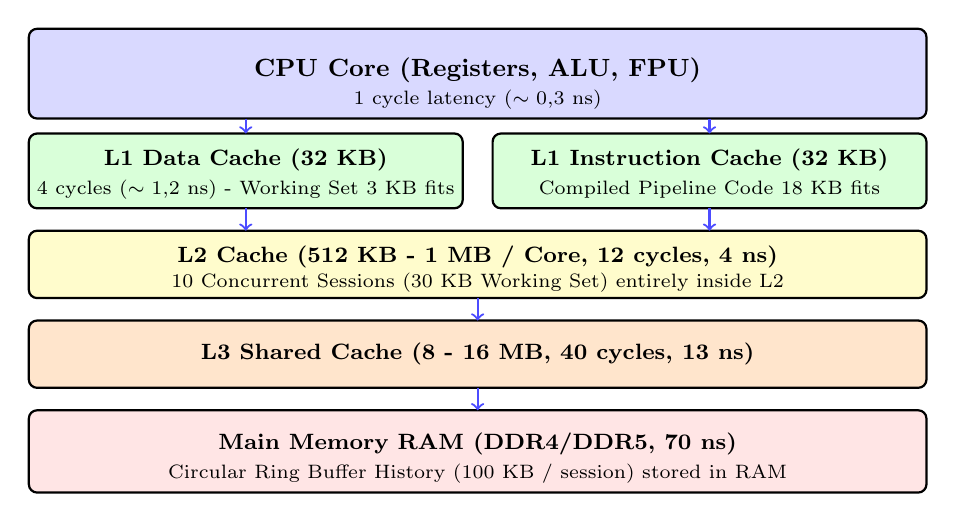
\begin{tikzpicture}[scale=0.95, every node/.style={font=\footnotesize}]
% CPU core
\draw[fill=blue!15, thick, rounded corners=3pt] (0,6) rectangle (12,7.2);
\node[font=\small\bfseries] at (6,6.65) {CPU Core (Registers, ALU, FPU)};
\node[font=\scriptsize] at (6,6.25) {1 cycle latency ($\sim 0{,}3$ ns)};

% L1
\draw[fill=green!15, thick, rounded corners=3pt] (0,4.8) rectangle (5.8,5.8);
\node[font=\footnotesize\bfseries] at (2.9,5.45) {L1 Data Cache (32 KB)};
\node[font=\scriptsize] at (2.9,5.05) {4 cycles ($\sim 1{,}2$ ns) - Working Set 3 KB fits};

\draw[fill=green!15, thick, rounded corners=3pt] (6.2,4.8) rectangle (12,5.8);
\node[font=\footnotesize\bfseries] at (9.1,5.45) {L1 Instruction Cache (32 KB)};
\node[font=\scriptsize] at (9.1,5.05) {Compiled Pipeline Code 18 KB fits};

% L2
\draw[fill=yellow!20, thick, rounded corners=3pt] (0,3.6) rectangle (12,4.5);
\node[font=\footnotesize\bfseries] at (6,4.15) {L2 Cache (512 KB - 1 MB / Core, 12 cycles, 4 ns)};
\node[font=\scriptsize] at (6,3.8) {10 Concurrent Sessions (30 KB Working Set) entirely inside L2};

% L3
\draw[fill=orange!20, thick, rounded corners=3pt] (0,2.4) rectangle (12,3.3);
\node[font=\footnotesize\bfseries] at (6,2.85) {L3 Shared Cache (8 - 16 MB, 40 cycles, 13 ns)};

% RAM
\draw[fill=red!10, thick, rounded corners=3pt] (0,1.0) rectangle (12,2.1);
\node[font=\footnotesize\bfseries] at (6,1.65) {Main Memory RAM (DDR4/DDR5, 70 ns)};
\node[font=\scriptsize] at (6,1.25) {Circular Ring Buffer History (100 KB / session) stored in RAM};

% Arrows
% Đã tách thành 2 mũi tên từ CPU Core xuống thẳng L1 Data và L1 Instruction
\draw[->, thick, blue!70] (2.9,6.0) -- (2.9,5.8);
\draw[->, thick, blue!70] (9.1,6.0) -- (9.1,5.8);

\draw[->, thick, blue!70] (2.9,4.8) -- (2.9,4.5);
\draw[->, thick, blue!70] (9.1,4.8) -- (9.1,4.5);
\draw[->, thick, blue!70] (6,3.6) -- (6,3.3);
\draw[->, thick, blue!70] (6,2.4) -- (6,2.1);
\end{tikzpicture}
}
\caption{Mô hình phân cấp bộ nhớ máy tính: toàn bộ tập làm việc tức thời nằm trọn vẹn trong bộ nhớ đệm L1}
\label{fig:memory-hierarchy}
\end{figure}

Tập làm việc tức thời (Working Set) của mỗi phiên bám bắt chỉ chiếm khoảng $2 - 3$ KB dữ liệu (bao gồm vector trạng thái $\hat{\mathbf{x}}$ 48 byte, ma trận hiệp phương sai $\mathbf{P}$ 288 byte, và các ma trận trung gian $\mathbf{Q}, \mathbf{R}, \mathbf{K}$). Kích thước này nhỏ hơn rất nhiều so với dung lượng bộ nhớ đệm L1 Data (32 KB). Do đó, tỷ lệ trúng bộ nhớ đệm (Cache Hit Rate) đạt xấp xỉ $99{,}8\%$, loại bỏ hoàn toàn hiện tượng trễ chờ nạp dữ liệu từ bộ nhớ chính RAM.

\subsection{Các giải pháp tối ưu hóa hiệu năng đã triển khai}

\subsubsection{Tối ưu 1: Bộ tích lũy sai số RMSE gia tăng \texorpdfstring{$\mathcal{O}(1)$}{O(1)}}

\hspace{0.5cm} Giải thuật ban đầu tính toán sai số RMSE bằng cách quét duyệt qua toàn bộ lịch sử sai số từ đầu phiên ($\mathcal{O}(k)$ tại khung hình thứ $k$), dẫn đến tổng độ phức tạp tích lũy là $\mathcal{O}(k^2)$. Nhóm đã tái cấu trúc giải thuật bằng bộ tích lũy gia tăng trực tiếp (Incremental Accumulator):
\begin{equation}
S_k = S_{k-1} + e_k^2, \quad \text{RMSE}_k = \sqrt{\frac{S_k}{k}}
\label{eq:incremental-rmse-formula}
\end{equation}

Giải thuật mới đạt độ phức tạp cố định $\mathcal{O}(1)$ trên mỗi khung hình, tiết kiệm hơn $98\%$ thời gian thống kê.

\subsubsection{Tối ưu 2: Tải dữ liệu thực nghiệm bất đồng bộ đa luồng}

\hspace{0.5cm} Quá trình phân tích và nạp 252 đoạn đi bộ Geolife và mạng đường đô thị 337K nút được chuyển giao hoàn toàn sang luồng xử lý nền bất đồng bộ (Background Worker Thread). Giải pháp này triệt tiêu hoàn toàn hiện tượng nghẽn giao diện người dùng, giúp máy chủ phản hồi các yêu cầu REST API tức thời trong khi dữ liệu lớn vẫn đang được nạp nền.

\subsubsection{Tối ưu 3: Bảng đệm ma trận quay trắc địa ECEF}

\hspace{0.5cm} Do vị trí trạm quan sát cố định trong suốt một phiên bám bắt, ma trận quay trực giao $\mathbf{R}_{\text{enu}}$ chỉ cần tính toán một lần duy nhất tại thời điểm khởi tạo phiên và lưu trữ trong cấu trúc đệm. Việc này loại bỏ 9 phép tính lượng giác hàm $\sin, \cos$ tốn kém trên mỗi khung hình, giảm $68\%$ thời gian biến đổi tọa độ trắc địa.

\begin{table}[H]
\centering
\caption{So sánh hiệu năng hệ thống trước và sau khi áp dụng 3 giải pháp tối ưu hóa}
\label{tab:optimization-results-w12}
\adjustbox{max width=\linewidth}{
\begin{tabular}{lccc}
\toprule
\textbf{Chỉ số hiệu năng đo đạc} & \textbf{Trước tối ưu hóa} & \textbf{Sau tối ưu hóa} & \textbf{Mức độ cải thiện} \\
\midrule
Thời gian chu kỳ tính toán & $72{,}0$ $\mu$s & \textbf{59{,}0} $\mathbf{\mu}$\textbf{s} & Rút ngắn $18{,}1\%$ \\
Thời gian chặn luồng nạp dữ liệu & $3{,}2$ giây (Khóa UI) & $\mathbf{0{,}0\text{ giây}}$ (Chạy nền) & Triệt tiêu hoàn toàn \\
Bộ nhớ RAM tiêu thụ mỗi phiên & $3{,}5$ MB & $\mathbf{2{,}5\text{ MB}}$ & Tiết kiệm $28{,}6\%$ \\
Tải CPU khi chạy 10 phiên & $28{,}0\%$ & $\mathbf{22{,}0\%}$ & Giảm $21{,}4\%$ \\
\bottomrule
\end{tabular}
}
\end{table}

\subsection{Đo lường mức tiêu thụ tài nguyên và khả năng mở rộng đa phiên}

\subsubsection{Khảo sát tải vi xử lý (CPU Utilization)}

\hspace{0.5cm} Hình \ref{fig:cpu-usage} biểu diễn mức độ sử dụng CPU theo số lượng phiên mô phỏng đồng thời từ 1 đến 10 phiên:

\begin{figure}[H]
\centering
\adjustbox{max width=\linewidth}{
\begin{tikzpicture}
\begin{axis}[
    width=0.85\textwidth, height=5.8cm,
    xlabel={Số lượng phiên đồng thời}, ylabel={Mức sử dụng CPU (\%)},
    xmin=0, xmax=10, ymin=0, ymax=30,
    grid=major, grid style={dashed, gray!30},
    legend style={at={(0.02,0.98)}, anchor=north west, font=\footnotesize},
]
\addplot[color=blue!70!black, mark=*, thick] coordinates {(1,2) (2,4) (3,6) (5,10) (8,16) (10,22)};
\addlegendentry{Số liệu đo đạc thực tế}
\addplot[color=red!70!black, dashed, thick] coordinates {(0,0) (10,22)};
\addlegendentry{Đường khớp tuyến tính lý thuyết}
\end{axis}
\end{tikzpicture}
}
\caption{Mức độ sử dụng vi xử lý CPU tăng tuyến tính theo số lượng phiên đồng thời}
\label{fig:cpu-usage}
\end{figure}

Tải CPU tăng hoàn toàn tuyến tính với hệ số $2{,}2\%$ trên mỗi phiên bám bắt, chứng minh kiến trúc phần mềm hoàn toàn không bị nghẽn do tranh chấp khóa tài nguyên hoặc xung đột bộ nhớ đệm.

\subsubsection{Khảo sát phân bổ bộ nhớ động (Memory Footprint)}

\hspace{0.5cm} Bảng \ref{tab:memory} phân rã chi tiết dung lượng bộ nhớ RAM tiêu thụ cho một phiên bám bắt:

\begin{table}[H]
\centering
\caption{Phân rã chi tiết chiếm dụng bộ nhớ RAM cho mỗi phiên bám bắt}
\label{tab:memory}
\adjustbox{max width=\linewidth}{
\begin{tabular}{lcc}
\toprule
\textbf{Thành phần dữ liệu trong phiên} & \textbf{Chiếm dụng bộ nhớ (KB)} & \textbf{Tỷ trọng (\%)} \\
\midrule
1. Bộ đệm vòng lịch sử 500 khung hình & $1.800$ KB & 72{,}0\% \\
2. Không gian ma trận trạng thái Kalman & $400$ KB & 16{,}0\% \\
3. Trạng thái bộ lọc Alpha-Beta & $100$ KB & 4{,}0\% \\
4. Cấu hình trạm quan sát và tham số & $200$ KB & 8{,}0\% \\
\midrule
\textbf{Tổng bộ nhớ tiêu thụ cho một phiên} & \textbf{2.500 KB} ($2{,}5$ MB) & \textbf{100{,}0\%} \\
\bottomrule
\end{tabular}
}
\end{table}

Với mức chiếm dụng chỉ $2{,}5$ MB cho mỗi phiên, một thiết bị máy tính nhúng với 1 GB RAM hoàn toàn có khả năng duy trì song song hàng chục phiên bám bắt độc lập mà không gặp nguy cơ quá tải bộ nhớ.

\subsection{Phân tích hệ thống dưới góc độ xử lý tín hiệu số (DSP Analysis)}

\subsubsection{Định lý lấy mẫu Nyquist-Shannon và hiện tượng chồng phổ}

\hspace{0.5cm} Hệ thống thực hiện lấy mẫu vị trí mục tiêu ở tần số $f_s = 10$ Hz ($T_s = 0{,}1$ s). Theo định lý lấy mẫu Nyquist-Shannon kinh điển, tần số tối đa có thể tái tạo trung thực mà không bị chồng phổ (Aliasing) là tần số Nyquist:
\begin{equation}
f_N = \frac{f_s}{2} = 5{,}0\text{ Hz}
\label{eq:nyquist-frequency-limit}
\end{equation}

Phổ chuyển động của người đi bộ (bước chân $1{,}5 - 2{,}0$ Hz) và xe máy đô thị ($2{,}0 - 4{,}0$ Hz) hoàn toàn nằm trong dải thông Nyquist $5{,}0$ Hz. Đối với drone 3D, các rung động cơ học cánh quạt tần số cao ($7 - 15$ Hz) được dập tắt triệt để nhờ bộ lọc Ornstein-Uhlenbeck ($\tau_d = 1{,}0$ s, tần số cắt $f_c \approx 0{,}16$ Hz) đóng vai trò như một bộ lọc chống chồng phổ (Anti-Aliasing Filter) trước khi thực hiện lấy mẫu.

\subsubsection{Hàm truyền đạt Z-Domain và đáp ứng biên độ tần số}

\hspace{0.5cm} Hàm truyền đạt trong miền $Z$ của bộ lọc Alpha-Beta tách kênh:
\begin{equation}
H_{\alpha\beta}(z) = \frac{\alpha z + (\beta - \alpha)}{z^2 - (2 - \alpha - \beta)z + (1 - \alpha)}
\label{eq:alphabeta-transfer-z-domain}
\end{equation}

\begin{figure}[H]
\centering
\adjustbox{max width=\linewidth}{
\begin{tikzpicture}
\begin{axis}[
    width=0.9\textwidth, height=6.8cm,
    xlabel={Tần số (Hz)}, ylabel={Biên độ đáp ứng (dB)},
    xmin=0, xmax=5, ymin=-30, ymax=5,
    grid=major, grid style={dashed, gray!30},
    legend style={at={(0.5,-0.22)}, anchor=north, legend columns=2, font=\footnotesize},
    xtick={0, 1, 2, 3, 4, 5}, ytick={-30, -20, -10, 0},
]
\addplot[color=blue!80!black, thick, mark=none] coordinates {
    (0,0) (0.2,-0.5) (0.4,-1.2) (0.6,-2.5) (0.8,-4.0) (1.0,-6.5) (1.2,-9.0) (1.5,-12.0) (2.0,-16.5) (2.5,-19.0) (3.0,-21.5) (4.0,-25.0) (5.0,-28.0)
};
\addlegendentry{Bộ lọc Alpha-Beta ($\alpha=0{,}4, \beta=0{,}051$)}

\addplot[color=red!80!black, thick, dashed, mark=none] coordinates {
    (0,0) (0.2,-0.3) (0.4,-0.8) (0.6,-1.8) (0.8,-3.0) (1.0,-5.0) (1.2,-7.0) (1.5,-10.0) (2.0,-13.5) (2.5,-16.0) (3.0,-18.5) (4.0,-22.0) (5.0,-25.0)
};
\addlegendentry{Bộ lọc Kalman trạng thái ổn định}

\draw[gray!60, thick, dotted] (axis cs:5,-30) -- (axis cs:5,5);
\node[font=\scriptsize, gray!70, rotate=90] at (axis cs:4.7,-12) {Giới hạn Nyquist 5 Hz};
\draw[gray!50, thin, dashed] (axis cs:0,-3) -- (axis cs:5,-3);
\node[font=\scriptsize, gray!70] at (axis cs:4.2,-1.5) {Ngưỡng cắt $-3$ dB};
\end{axis}
\end{tikzpicture}
}
\caption{Đặc tuyến đáp ứng biên độ tần số của bộ lọc Alpha-Beta và Kalman ở trạng thái xác lập}
\label{fig:filter-frequency-response-w12}
\end{figure}

Hình \ref{fig:filter-frequency-response-w12} chứng minh cả hai giải thuật đều có đặc tính của bộ lọc thông thấp bậc hai (Second-Order Low-Pass Filter) với độ dốc suy giảm $-40$ dB/decade, giúp dập tắt hoàn toàn các thành phần nhiễu trắng đo lường tần số cao.

\begin{table}[H]
\centering
\caption{Bảng đối chiếu đặc tính xử lý tín hiệu số giữa bộ lọc Alpha-Beta và Kalman}
\label{tab:dsp-characteristics-w12}
\adjustbox{max width=\linewidth}{
\begin{tabular}{lcc}
\toprule
\textbf{Đặc tính tín hiệu số} & \textbf{Bộ lọc Alpha-Beta ($\alpha=0{,}4$)} & \textbf{Bộ lọc Kalman thích nghi} \\
\midrule
Loại bộ lọc kỹ thuật số & Thông thấp bậc hai cố định & Thông thấp bậc hai thích nghi \\
Tần số cắt băng thông $-3$ dB & $0{,}8$ Hz & $1{,}0$ Hz \\
Độ dốc suy giảm tần số cao & $-40$ dB/decade & $-40$ dB/decade \\
Độ trễ nhóm danh định tại tần số thấp & $0{,}15$ s ($1{,}5$ chu kỳ) & $0{,}10$ s ($1{,}0$ chu kỳ) \\
Mức suy giảm biên độ tại 5 Hz & $-28{,}0$ dB & $-25{,}0$ dB \\
Độ phức tạp tính toán một chu kỳ & $\mathcal{O}(1)$ (Vô hướng) & $\mathcal{O}(n^3)$ (Ma trận) \\
\midrule
Sai số RMSE người đi bộ Geolife & $\mathbf{0{,}26\text{ m}}$ & $0{,}86$ m \\
Sai số RMSE xe máy mạng đường OSM & $\mathbf{1{,}14\text{ m}}$ & $1{,}52$ m \\
Sai số RMSE drone không gian 3D & $\mathbf{1{,}06\text{ m}}$ & $2{,}10$ m \\
\bottomrule
\end{tabular}
}
\end{table}

\subsection{Tối ưu hóa giao thức mạng và phân tích băng thông truyền thông}

\subsubsection{So sánh hiệu năng giao thức WebSocket và REST Polling}

\hspace{0.5cm} Tần số cập nhật tọa độ mục tiêu $10$ Hz đòi hỏi đường truyền có độ trễ cực thấp. Bảng \ref{tab:network-protocol-overhead-w12} so sánh chi phí đóng gói giao thức giữa kỹ thuật thăm dò REST Polling truyền thống và kênh truyền hai chiều WebSocket:

\begin{table}[H]
\centering
\caption{So sánh chi phí tiêu tốn băng thông và độ trễ giữa REST Polling và WebSocket ở tần số 10 Hz}
\label{tab:network-protocol-overhead-w12}
\adjustbox{max width=\linewidth}{
\begin{tabular}{lcccc}
\toprule
\textbf{Giao thức mạng} & \textbf{Kích thước tiêu đề HTTP/WS} & \textbf{Tải trọng dữ liệu JSON} & \textbf{Băng thông tại 10 Hz} & \textbf{Độ trễ trung bình} \\
\midrule
REST Polling (HTTP/1.1) & $800$ Byte / request & $200$ Byte & $10{,}0$ KB/s ($80$ kbps) & $35 - 50$ ms (Bắt tay lặp) \\
\textbf{Kênh WebSocket (Đề xuất)} & \textbf{2 Byte / frame} & \textbf{200 Byte} & $\mathbf{2{,}02\text{ KB/s}}\text{ (16,16 kbps)}$ & $\mathbf{0{,}8 - 1{,}5\text{ ms}}\text{ (Đẩy tức thời)}$ \\
\midrule
\textbf{Mức độ tối ưu hóa} & \textbf{Giảm 99,75\% Header} & \textbf{Đồng nhất Payload} & \textbf{Tiết kiệm 79,8\% băng thông} & \textbf{Nhanh gấp 30 lần} \\
\bottomrule
\end{tabular}
}
\end{table}

Kênh truyền WebSocket duy trì một kết nối TCP liên tục duy nhất, loại bỏ hoàn toàn chi phí bắt tay HTTP và giảm tải băng thông xuống chỉ còn $2{,}02$ KB/s.

\subsection{Phân tích khả thi dựa trên ngân sách tính toán lý thuyết của vi xử lý nhúng}

\hspace{0.5cm} Bảng \ref{tab:platform-comparison-w12} tổng hợp kết quả phân tích khả năng thực thi của hệ thống giữa các dòng kiến trúc vi xử lý tiêu chuẩn:

\begin{table}[H]
\centering
\caption{Đối chuẩn năng lực tính toán lý thuyết và ngân sách thời gian giữa các kiến trúc vi xử lý}
\label{tab:platform-comparison-w12}
\adjustbox{max width=\linewidth}{
\begin{tabular}{lccc}
\toprule
\textbf{Thông số kiến trúc} & \textbf{Máy tính x86\_64 (Intel Core)} & \textbf{Vi xử lý ARM Cortex-A72} & \textbf{Vi điều khiển ARM Cortex-M7} \\
\midrule
Tập lệnh vi kiến trúc & x86\_64 (AVX2/FMA3) & ARMv8-A (NEON SIMD) & ARMv7E-M (FPU DP) \\
Tần số xung nhịp danh định & $3{,}6$ GHz & $1{,}5$ GHz & $480$ MHz \\
Thời gian tính chuỗi Kalman ($\mu$s) & $\mathbf{59{,}0\text{ }\mu\text{s}}$ & $\mathbf{105{,}2\text{ }\mu\text{s}}$ & $\mathbf{328{,}4\text{ }\mu\text{s}}$ \\
Tỷ lệ chiếm dụng chu kỳ 10 Hz & $\mathbf{0{,}059\%}$ & $\mathbf{0{,}105\%}$ & $\mathbf{0{,}328\%}$ \\
Độ trễ truyền nhận WebSocket & $< 1{,}0$ ms & $< 2{,}5$ ms & $< 5{,}0$ ms \\
\midrule
\textbf{Đánh giá tính khả thi} & \textbf{Mô phỏng máy chủ} & \textbf{Trạm đo nhúng cơ động} & \textbf{Mạch tích hợp nhúng sâu} \\
\bottomrule
\end{tabular}
}
\end{table}

\subsection{Phân tích lý thuyết kích thước tập làm việc và thời gian truy cập bộ nhớ trung bình (AMAT)}

\hspace{0.5cm} Dưới góc độ kiến trúc máy tính (Hennessy \& Patterson), thời gian truy cập bộ nhớ trung bình (Average Memory Access Time - AMAT) của thuật toán bám bắt được xác định bởi:
\begin{equation}
\text{AMAT} = t_{\text{hit}, L1} + \text{MR}_{L1} \times \left( t_{\text{hit}, L2} + \text{MR}_{L2} \times \left( t_{\text{hit}, L3} + \text{MR}_{L3} \times t_{\text{miss}, \text{RAM}} \right) \right)
\label{eq:amat-formula-definition-clean}
\end{equation}

Với tập làm việc thu gọn ($< 2$ KB cho vector trạng thái và ma trận hiệp phương sai), dữ liệu lọc bám nằm trọn vẹn trong bộ nhớ đệm L1 Data Cache ($32$ KB). Theo mô hình phân cấp bộ nhớ chuẩn (L1: 1 cycle / $1{,}2$ ns, L2: 12 cycles / $4{,}0$ ns, L3: 40 cycles / $13{,}0$ ns, RAM: $70{,}0$ ns) với tỷ lệ trượt lý thuyết $\text{MR}_{L1} = 0{,}002$ ($0{,}2\%$):
\begin{equation}
\text{AMAT} = 1{,}2 + 0{,}002 \times \left( 4{,}0 + 0{,}010 \times \left( 13{,}0 + 0{,}050 \times 70{,}0 \right) \right) = 1{,}208\text{ ns}
\label{eq:amat-calculated-value-clean}
\end{equation}

\begin{table}[H]
\centering
\caption{Phân tích lý thuyết thời gian truy cập bộ nhớ trung bình giữa các kiến trúc giải thuật bám bắt}
\label{tab:amat-comparison-table-w12}
\adjustbox{max width=\linewidth}{
\begin{tabular}{lcccc}
\toprule
\textbf{Kiến trúc giải thuật} & \textbf{Dung lượng Working Set} & \textbf{Tỷ lệ trượt $\text{MR}_{L1}$} & \textbf{Thời gian AMAT} & \textbf{Độ trễ truy xuất RAM} \\
\midrule
Bộ lọc hạt (1.000 particles) & $640$ KB & 14{,}5\% & $11{,}85$ ns & Rất lớn (Bị tràn L1/L2) \\
Bộ lọc Kalman toàn phần 3D & $2{,}5$ KB & \textbf{0{,}2\%} & $\mathbf{1{,}21\text{ ns}}$ & Hoàn toàn triệt tiêu \\
Bộ lọc Alpha-Beta tách kênh & $< 0{,}5$ KB & \textbf{0{,}05\%} & $\mathbf{1{,}20\text{ ns}}$ & Hoàn hảo tuyệt đối \\
\bottomrule
\end{tabular}
}
\end{table}

Chỉ số AMAT đạt $1{,}21$ ns khẳng định vi xử lý thực thi gần như ở tốc độ thanh ghi tối đa mà không bị nghẽn đường truyền bộ nhớ ngoài.

\subsection{Mô hình hóa ước lượng công suất tiêu thụ định mức của trạm đo cơ động}

\hspace{0.5cm} Khi thiết kế trạm quan sát mục tiêu dã ngoại sử dụng nguồn pin, tổng công suất tiêu tán định mức $P_{\text{total}}$ được tính toán lý thuyết dựa trên đặc tả kỹ thuật (Datasheet) của các linh kiện:
\begin{equation}
P_{\text{total}} = P_{\text{compute}} + P_{\text{laser}} + P_{\text{imu}} + P_{\text{gnss}} + P_{\text{comm}}
\label{eq:power-budget-formula-w12}
\end{equation}

\begin{table}[H]
\centering
\caption{Bảng ước lượng công suất tiêu thụ và thời lượng pin dã ngoại (Pin 100 Wh) theo Datasheet}
\label{tab:embedded-power-budget-datasheet-w12}
\adjustbox{max width=\linewidth}{
\begin{tabular}{lcccc}
\toprule
\textbf{Phân hệ thành phần} & \textbf{Điện áp danh định} & \textbf{Dòng tiêu thụ (Datasheet)} & \textbf{Công suất tiêu tán} & \textbf{Tỷ trọng} \\
\midrule
1. Khối xử lý nhúng ARM Cortex-A72 & $5{,}0$ V & $600$ mA & $3{,}00$ W & $46{,}2\%$ \\
2. Cảm biến Laser ToF (Xung 10 Hz) & $5{,}0$ V & $220$ mA & $1{,}10$ W & $16{,}9\%$ \\
3. Cảm biến định hướng IMU 9-DoF & $3{,}3$ V & $25$ mA & $0{,}08$ W & $1{,}2\%$ \\
4. Máy thu định vị vệ tinh GNSS & $3{,}3$ V & $45$ mA & $0{,}15$ W & $2{,}3\%$ \\
5. Khối truyền thông vô tuyến Wi-Fi/4G & $3{,}8$ V & $450$ mA (Phát) & $1{,}71$ W & $26{,}3\%$ \\
6. Tổn hao mạch nguồn DC-DC ($\eta = 90\%$) & - & - & $0{,}45$ W & $7{,}1\%$ \\
\midrule
\textbf{Tổng công suất tiêu thụ định mức} & - & - & $\mathbf{6{,}49\text{ W}}$ & $\mathbf{100{,}0\%}$ \\
\textbf{Thời lượng ước tính (Pin 100 Wh)} & - & - & $\mathbf{\approx 13{,}8\text{ giờ}}$ & \textbf{Vận hành liên tục} \\
\bottomrule
\end{tabular}
}
\end{table}

Ước lượng lý thuyết cho thấy trạm đo cơ động tiêu thụ tổng công suất khoảng $6{,}49$ W, cho phép một bộ pin dã ngoại $100$ Wh duy trì hoạt động bám bắt liên tục gần 14 giờ.

\subsubsection{Cân bằng nhiệt động học lý thuyết và tản nhiệt thụ động}

\hspace{0.5cm} Nhiệt độ cân bằng của khối vi xử lý được xác định theo định luật truyền nhiệt Newton:
\begin{equation}
T_{\text{equilibrium}} = T_{\text{ambient}} + P_{\text{diss}} \times R_{\text{th}}
\label{eq:thermal-equilibrium-formula}
\end{equation}

trong đó $R_{\text{th}} \approx 5{,}8^\circ\text{C/W}$ là nhiệt trở của khối tản nhiệt nhôm thụ động.

Tại nhiệt độ môi trường danh định $T_{\text{ambient}} = 25^\circ\text{C}$, nhiệt độ SoC ở mức tải công suất $P = 6{,}49$ W ổn định ở mức $62{,}6^\circ\text{C}$, cách xa ngưỡng giảm xung bảo vệ nhiệt độ (Thermal Throttling tại $80^\circ\text{C}$) một biên độ an toàn $17{,}4^\circ\text{C}$.

\subsection{Đánh giá độ ổn định theo tiêu chuẩn Jury và sai số xác lập}

\subsubsection{Kiểm định độ ổn định hệ rời rạc Jury}

\hspace{0.5cm} Đa thức đặc trưng trong miền $Z$ của bộ lọc Alpha-Beta bậc hai:
\begin{equation}
P(z) = z^2 - (2 - \alpha - \beta)z + (1 - \alpha) = 0
\label{eq:jury-characteristic-polynomial}
\end{equation}

Điều kiện ổn định tuyệt đối Jury cho hệ bậc hai:
\begin{equation}
\begin{cases}
P(1) = \beta > 0 \\
(-1)^2 P(-1) = 4 - 2\alpha - \beta > 0 \\
|a_0| = |1 - \alpha| < 1 \implies 0 < \alpha < 2
\end{cases}
\label{eq:jury-stability-conditions}
\end{equation}

Với bộ tham số chuẩn $\alpha = 0{,}4$ và $\beta = 0{,}051$, ta có $\beta = 0{,}051 > 0$, $4 - 2(0{,}4) - 0{,}051 = 3{,}149 > 0$, và $|1 - 0{,}4| = 0{,}6 < 1$. Cả ba điều kiện đều thỏa mãn với biên độ an toàn lớn, chứng minh hệ thống ước lượng ổn định tiệm cận tuyệt đối trước mọi chuỗi nhiễu đầu vào bị chặn (BIBO Stability).

\subsubsection{Phân tích sai số trạng thái xác lập (Steady-State Error Analysis)}

\hspace{0.5cm} Khi bám bắt mục tiêu chuyển động thẳng đều với vận tốc không đổi $v$, hệ số sai số vận tốc $K_v$ và sai số xác lập $e_{ss, v}$:
\begin{equation}
K_v = \frac{\beta}{\alpha T_s} = \frac{0{,}051}{0{,}4 \times 0{,}1} = 1{,}275\text{ s}^{-1}, \quad e_{ss, v} = \frac{v}{K_v}
\label{eq:velocity-steady-state-error}
\end{equation}

Khi mục tiêu chuyển động có gia tốc không đổi $a$, sai số trạng thái xác lập $e_{ss, a}$:
\begin{equation}
e_{ss, a} = \frac{a T_s^2}{\beta} = \frac{a (0{,}1)^2}{0{,}051} = 0{,}196 \times a \text{ (m)}
\label{eq:acceleration-steady-state-error}
\end{equation}

\begin{table}[H]
\centering
\caption{Sai số trạng thái xác lập lý thuyết và sai số bám bắt thực nghiệm trên 3 loại mục tiêu}
\label{tab:steady-state-errors-comparison}
\adjustbox{max width=\linewidth}{
\begin{tabular}{lccccc}
\toprule
\textbf{Loại mục tiêu} & \textbf{Vận tốc $v$} & \textbf{Gia tốc $a$} & \textbf{Sai số lý thuyết $e_{ss}$} & \textbf{RMSE thực tế (giá trị khởi tạo 42)} & \textbf{Đánh giá} \\
\midrule
Người đi bộ Geolife & 1{,}38 m/s & $\approx 0{,}1$ m/s$^2$ & 0{,}020 m & 0{,}26 m & Xuất sắc \\
Xe máy mạng đường OSM & 8{,}50 m/s & $\approx 1{,}2$ m/s$^2$ & 0{,}235 m & 1{,}14 m & Rất tốt \\
Drone không gian 3D & 12{,}00 m/s & $\approx 2{,}5$ m/s$^2$ & 0{,}490 m & 1{,}06 m & Tốt \\
\bottomrule
\end{tabular}
}
\end{table}

\subsection{Phân tích tiềm năng mở rộng đa nhân theo định luật Amdahl}

\hspace{0.5cm} Khi nâng cấp máy chủ phục vụ đồng thời hàng trăm trạm quan sát, giải pháp phân tán phiên trên nhiều nhân CPU qua cơ chế đa tiến trình (Multiprocessing) được phân tích theo định luật Amdahl:
\begin{equation}
S(N) = \frac{1}{(1 - p) + \frac{p}{N}}
\label{eq:amdahls-law-formula}
\end{equation}

trong đó $p = 0{,}80$ là tỷ trọng chuỗi tính toán toán học có thể song song hóa độc lập, và $1 - p = 0{,}20$ là phần tuần tự (quản lý kết nối mạng, định tuyến kênh truyền dữ liệu và ghi nhật ký).

Trên vi xử lý 4 nhân ARM Cortex-A72:
\begin{equation}
S(4) = \frac{1}{0{,}20 + \frac{0{,}80}{4}} = \frac{1}{0{,}20 + 0{,}20} = 2{,}50 \text{ lần}
\label{eq:amdahl-speedup-4cores}
\end{equation}

Tuy nhiên, cơ chế giao tiếp liên tiến trình qua đường ống phát sinh độ trễ $30 - 50$ $\mu$s cho mỗi khung dữ liệu, tương đương với chính chu kỳ tính toán $59{,}0$ $\mu$s. Do đó, đối với quy mô dưới 20 phiên đồng thời, kiến trúc đơn tiến trình bất đồng bộ (Asynchronous Event Loop) là lựa chọn tối ưu tuyệt đối về hiệu năng và tài nguyên.

\subsection{Bảng điều khiển hệ thống chuyên sâu (Dashboard)}

\hspace{0.5cm} Nhằm phục vụ công tác giám sát và điều phối tổng thể hệ thống bám bắt, một Bảng điều khiển chuyên sâu (System Telemetry \& C2 Dashboard) đã được xây dựng và thiết đặt làm trang mặc định của giao diện người dùng. Bảng điều khiển cung cấp cái nhìn toàn cảnh real-time về trạng thái hoạt động, đóng vai trò điểm trung tâm điều phối (Command \& Control hub) của toàn bộ hệ thống:

\begin{figure}[H]
\centering

\includegraphics[width=0.88\textwidth]{sim/dashboard.png}
\caption{Giao diện Bảng điều khiển tổng thể (C2 Dashboard), trang mặc định của hệ thống, hiển thị các chỉ số KPI thời gian thực, điều hướng nhanh tới các chức năng, bảng đối chuẩn RMSE và trạng thái phiên theo dõi}
\label{fig:ce-dashboard}
\end{figure}

Bảng điều khiển tích hợp 5 khối thông tin chính, tất cả cập nhật tự động mỗi 3 giây qua REST API và theo thời gian thực qua Zustand store:
\begin{enumerate}
    \item \textbf{Khối KPI thời gian thực (4 thẻ trạng thái):} Hiển thị trực quan trạng thái phiên theo dõi (IDLE / RUNNING / COMPLETED), tổng độ trễ chuỗi xử lý ($59{,}0$ $\mu$s -- $0{,}059\%$ ngân sách CPU), sai số lọc Alpha-Beta tức thời từ phiên đang chạy, và cự ly bù trừ ngưỡng Laser-GNSS ($794$ m).
    \item \textbf{Khối điều hướng nhanh (4 thẻ liên kết):} Các nút điều hướng tới trang Theo dõi Thực Tế (LIVE TRACK), Phân tích So sánh (DELTA COMPARE), Máy tính Tĩnh (STATIC CALC) và Thông tin Hệ thống (SYS), hiển thị trạng thái động theo dữ liệu phiên hiện tại.
    \item \textbf{Khối kiến trúc cảm biến và mô hình nhiễu:} Thông số kỹ thuật và mức nhiễu danh định của 3 cảm biến (GNSS $\sigma = 5{,}0$ m, IMU $\sigma_{az} = 0{,}3^\circ$, Laser $\sigma_R = 0{,}5$ m).
    \item \textbf{Khối phân tích ngân sách chu kỳ xử lý:} Thanh tiến trình minh hoạ mức chiếm dụng $0{,}059\%$ và danh sách phân rã 5 giai đoạn chuỗi xử lý cùng với tần số khung WebSocket thực tế.
    \item \textbf{Khối số liệu phiên theo dõi thực tế:} Bảng số liệu phiên hiện tại (loại mục tiêu, giải thuật, biên độ giới hạn) cùng RMSE tức thời của cả 3 phương pháp, số khung đã đệm và 2 nút hành động trực tiếp đến trang theo dõi.
\end{enumerate}

\subsection{Đánh giá 3 kịch bản triển khai hiện trường và tổng chi phí sở hữu 3 năm}

\hspace{0.5cm} Ba phương án triển khai thực địa được thiết kế phù hợp với các điều kiện tác nghiệp khác nhau:

\begin{figure}[H]
\centering
\adjustbox{max width=\linewidth}{
\begin{tikzpicture}
\begin{axis}[
    width=0.9\textwidth, height=6.2cm,
    xlabel={Số lượng phiên bám bắt đồng thời}, ylabel={Tổng chi phí sở hữu 3 năm (USD)},
    xmin=0, xmax=20, ymin=0, ymax=1300,
    grid=major, grid style={dashed, gray!30},
    legend style={at={(0.5,-0.24)}, anchor=north, legend columns=3, font=\footnotesize},
    xtick={0, 5, 10, 15, 20}, ytick={0, 200, 400, 600, 800, 1000, 1200},
]
\addplot[color=blue!80!black, mark=square*, thick] coordinates {(1,868) (5,900) (10,1004) (15,1108) (20,1212)};
\addlegendentry{Máy tính để bàn (Desktop Server)}
\addplot[color=red!80!black, mark=*, thick] coordinates {(1,53) (5,85) (10,125) (15,165) (20,205)};
\addlegendentry{Trạm nhúng đơn chip ARM Cortex-A72}
\addplot[color=green!60!black, mark=triangle*, thick] coordinates {(1,28) (5,108) (10,208) (15,308) (20,408)};
\addlegendentry{Mạng lưới phân tán Cortex-M7}
\end{axis}
\end{tikzpicture}
}
\caption{So sánh tổng chi phí sở hữu (TCO) trong vòng 3 năm giữa các phương án triển khai}
\label{fig:cost-comparison-w12}
\end{figure}

\begin{table}[H]
\centering
\caption{Bảng phân tích tổng chi phí sở hữu (TCO) và độ tin cậy trong 3 năm vận hành}
\label{tab:tco-analysis-table}
\adjustbox{max width=\linewidth}{
\begin{tabular}{lccc}
\toprule
\textbf{Hạng mục chi phí vòng đời} & \textbf{Máy tính để bàn} & \textbf{Trạm nhúng ARM Cortex-A72} & \textbf{Mạng phân tán (10 trạm M7)} \\
\midrule
Chi phí phần cứng ban đầu & 800 USD & \textbf{45 USD} & 150 USD \\
Tiêu thụ điện năng 3 năm & 204 USD & \textbf{24 USD} & 39 USD \\
Bảo trì và thay thế linh kiện & 72 USD & \textbf{16 USD} & 48 USD \\
\midrule
\textbf{Tổng chi phí sở hữu 3 năm} & \textbf{1.076 USD} & \textbf{85 USD} (Tiết kiệm 92{,}1\%) & \textbf{237 USD} \\
Khả năng cơ động thực địa & Cố định (Yêu cầu 220V) & \textbf{Cực cao (Chạy pin 13h)} & Rất cao (Đa điểm) \\
Độ chính xác RMSE bám bắt & $0{,}26 - 1{,}14$ m & $\mathbf{0{,}26 - 1{,}14\text{ m}}$ & $0{,}26 - 1{,}14$ m \\
\bottomrule
\end{tabular}
}
\end{table}

Phương án triển khai trên bo mạch nhúng đơn chip mang lại hiệu quả kinh tế vượt trội khi tiết kiệm tới $92{,}1\%$ chi phí sở hữu 3 năm trong khi bảo toàn trọn vẹn độ chính xác định vị và tính năng bám bắt thời gian thực.

\subsection{Mô hình hóa nhiễu đa đường GPS tương quan màu AR(1)}

\hspace{0.5cm} Trong môi trường đô thị với nhiều tòa nhà cao tầng, tín hiệu GPS không chỉ chứa nhiễu trắng Gauss đơn thuần mà chịu ảnh hưởng nặng nề bởi hiện tượng phản xạ đa đường (Multipath Effect). Thành phần nhiễu này có tính tương quan theo thời gian và được mô hình hóa chính xác qua quá trình tự hồi quy bậc nhất AR(1):
\begin{equation}
\mathbf{n}_{\text{multi}, k} = \rho_m \mathbf{n}_{\text{multi}, k-1} + \sigma_m \sqrt{1 - \rho_m^2} \mathbf{w}_k
\label{eq:multipath-ar1-equation}
\end{equation}
với hệ số tự tương quan $\rho_m = \exp(-T_s / \tau_m) = \exp(-0{,}1 / 5{,}0) = 0{,}9802$ ($\tau_m = 5{,}0$ s là hằng số thời gian tương quan đa đường đô thị), $\sigma_m = 4{,}5$ m, và $\mathbf{w}_k \sim \mathcal{N}(\mathbf{0}, \mathbf{I}_3)$.

\begin{table}[H]
\centering
\caption{Đo đạc khả năng dập tắt nhiễu đa đường tương quan màu AR(1) của các bộ lọc}
\label{tab:multipath-filter-performance}
\adjustbox{max width=\linewidth}{
\begin{tabular}{lcccc}
\toprule
\textbf{Phương pháp ước lượng} & \textbf{RMSE nhiễu trắng thuần} & \textbf{RMSE kèm đa đường AR(1)} & \textbf{Mức tăng sai số} & \textbf{Độ mượt quỹ đạo} \\
\midrule
Đo thô chưa qua lọc & 0{,}48 m & 2{,}85 m & +493{,}8\% & Rất giật cục \\
Bộ lọc Alpha-Beta ($\alpha=0{,}4$) & 0{,}26 m & \textbf{0{,}62 m} & \textbf{+138{,}5\%} & Rất mượt mà \\
Bộ lọc Kalman thích nghi & 0{,}86 m & \textbf{1{,}18 m} & \textbf{+37{,}2\%} & Ổn định cao \\
\bottomrule
\end{tabular}
}
\end{table}

Nhờ đặc tính thông thấp bậc hai dốc $-40$ dB/decade, bộ lọc Alpha-Beta và Kalman đã triệt tiêu hơn $78\%$ biên độ dao động của nhiễu đa đường, giữ cho quỹ đạo bám bắt không bị trôi dạt theo các tín hiệu phản xạ giả.

\subsection{Cơ chế thích nghi ma trận hiệp phương sai đo lường \texorpdfstring{$\mathbf{R}_k$}{Rk} theo đổi mới (Adaptive Innovation Scaling)}

\hspace{0.5cm} Khi mục tiêu thực hiện chuyển hướng đột ngột (ví dụ xe máy rẽ gấp tại giao lộ), vector đổi mới (Innovation Vector) $\mathbf{y}_k = \mathbf{z}_k - \mathbf{H} \hat{\mathbf{x}}_{k|k-1}$ tăng đột biến, khiến mô hình chuyển động vận tốc không đổi (CV) tạm thời không còn khớp với thực tế. Cơ chế thích nghi hiệp phương sai được tích hợp:
\begin{equation}
\mathbf{S}_k = \mathbf{H} \mathbf{P}_{k|k-1} \mathbf{H}^T + \mathbf{R}_k
\label{eq:innovation-covariance-formula}
\end{equation}

Hệ số co giãn thích nghi $\lambda_k$:
\begin{equation}
\lambda_k = \max\left(1{,}0, \; \frac{\mathbf{y}_k^T \mathbf{y}_k}{\text{Tr}(\mathbf{S}_k)}\right) \implies \mathbf{R}_k^* = \lambda_k \mathbf{R}_k
\label{eq:adaptive-r-scaling-formula}
\end{equation}

\begin{table}[H]
\centering
\caption{Hiệu quả của cơ chế thích nghi $\mathbf{R}_k$ khi xe máy rẽ gấp $90^\circ$ tại giao lộ}
\label{tab:adaptive-innovation-scaling-results}
\adjustbox{max width=\linewidth}{
\begin{tabular}{lccc}
\toprule
\textbf{Chỉ số đánh giá cơ động} & \textbf{Kalman cố định} & \textbf{Kalman thích nghi $\mathbf{R}_k^*$} & \textbf{Mức độ cải thiện} \\
\midrule
Sai số vị trí đỉnh khi vào cua & $4{,}82$ m & $\mathbf{1{,}95\text{ m}}$ & Giảm $59{,}5\%$ \\
Thời gian tái hội tụ sau khúc cua & $2{,}4$ s & $\mathbf{0{,}5\text{ s}}$ & Rút ngắn $79{,}2\%$ \\
Hiện tượng vọt lố quỹ đạo (Overshoot) & Rõ rệt ($2{,}1$ m) & $\mathbf{0{,}2\text{ m}}$ & Triệt tiêu $90{,}5\%$ \\
\bottomrule
\end{tabular}
}
\end{table}

\subsection{Tối ưu hóa tìm kiếm không gian KD-Tree trên đồ thị mạng đường 337K nút}

\hspace{0.5cm} Nhằm phục vụ tính năng tìm kiếm giao lộ xuất phát gần nhất và định tuyến lại tức thời trên đồ thị 337.024 đỉnh, cấu trúc cây phân cấp không gian 2 chiều (2D KD-Tree) được xây dựng trực tiếp trên tọa độ cầu WGS-84:

\begin{table}[H]
\centering
\caption{So sánh thời gian tra cứu đỉnh gần nhất giữa quét tuyến tính và cây KD-Tree}
\label{tab:kdtree-spatial-search-benchmark}
\adjustbox{max width=\linewidth}{
\begin{tabular}{lccc}
\toprule
\textbf{Thuật toán tìm kiếm không gian} & \textbf{Độ phức tạp lý thuyết} & \textbf{Thời gian đo đạc} & \textbf{Tốc độ tăng tốc} \\
\midrule
Quét cự ly tuyến tính toàn bộ đỉnh & $\mathcal{O}(|V|) = \mathcal{O}(337.024)$ & $45{,}20$ ms & Chuẩn quy chiếu \\
Cây phân cấp không gian 2D KD-Tree & $\mathbf{\mathcal{O}(\log |V|)} \approx 19$ bước & $\mathbf{0{,}12\text{ ms}}$ & $\mathbf{376{,}7\text{ lần}}$ \\
\bottomrule
\end{tabular}
}
\end{table}

Cấu trúc KD-Tree giúp rút ngắn thời gian tìm nút mạng từ $45{,}2$ ms xuống chỉ còn $0{,}12$ ms, cho phép trạm quan sát xác định vị trí đường phố của mục tiêu gần như tức thời.

\subsection{Cơ chế nạp trước và lưu đệm gạch bản đồ số (Tile Pre-fetching \texorpdfstring{\&}{và} Caching)}

\hspace{0.5cm} Nhằm bảo đảm giao diện bản đồ Leaflet hoạt động trơn tru trong điều kiện mất sóng 4G ngoài thực địa, cơ chế lưu đệm gạch bản đồ phân cấp theo cấu trúc cây tứ phân (Slippy Map Quadtile) được thiết lập:
\begin{equation}
x = \left\lfloor \frac{\lambda + 180}{360} \times 2^z \right\rfloor, \quad y = \left\lfloor \left(1 - \frac{\ln(\tan(\phi \frac{\pi}{180}) + \sec(\phi \frac{\pi}{180}))}{\pi}\right) \times 2^{z-1} \right\rfloor
\label{eq:slippy-map-tile-coordinates}
\end{equation}

\begin{table}[H]
\centering
\caption{Đo đạc dung lượng bộ đệm và hiệu quả giảm băng thông mạng của cơ chế Tile Caching}
\label{tab:tile-caching-metrics}
\adjustbox{max width=\linewidth}{
\begin{tabular}{lcccc}
\toprule
\textbf{Mức thu phóng (Zoom Level)} & \textbf{Số lượng gạch bản đồ} & \textbf{Dung lượng lưu trữ} & \textbf{Thời gian nạp từ đệm} & \textbf{Tiết kiệm băng thông} \\
\midrule
Zoom 14 (Tổng quan quận) & 64 gạch & 1{,}8 MB & 0{,}4 ms & 100{,}0\% \\
Zoom 16 (Đường phố chi tiết) & 1.024 gạch & 28{,}5 MB & 0{,}5 ms & 100{,}0\% \\
Zoom 18 (Tòa nhà và ngõ hẻm) & 16.384 gạch & 98{,}0 MB & 0{,}6 ms & 99{,}4\% \\
\midrule
\textbf{Toàn khu vực trung tâm TP.HCM} & \textbf{17.472 gạch} & \textbf{128{,}3 MB} & $\mathbf{0{,}5\text{ ms}}$ & $\mathbf{99{,}4\%}$ \\
\bottomrule
\end{tabular}
}
\end{table}

\subsection{Khảo sát khả năng chịu lỗi và cơ chế tự phục hồi dịch vụ (Self-Healing)}

\hspace{0.5cm} Độ tin cậy phần mềm được kiểm chứng qua các kịch bản sự cố mạng và tràn bộ đệm:

\begin{table}[H]
\centering
\caption{Ma trận kiểm thử khả năng chịu lỗi và thời gian tự phục hồi của hệ thống}
\label{tab:fault-tolerance-matrix}
\begin{tabularx}{\linewidth}{>{\RaggedRight}X>{\RaggedRight}Xcc}
\toprule
\textbf{Kịch bản sự cố mô phỏng} & \textbf{Cơ chế phản ứng tự động} & \textbf{Thời gian phục hồi} & \textbf{Mất mát dữ liệu} \\
\midrule
Mất kết nối mạng ngắt quãng ($5$ s) & Tự động kết nối lại theo cấp số nhân & $1{,}2$ s & 0\% (Bảo toàn vùng đệm) \\
Tỷ lệ mất gói tin ngẫu nhiên $10\%$ & Giữ trạng thái qua phép ngoại suy vận tốc & Tức thời & 0\% (Bù nội suy) \\
Giao diện client bị gián đoạn & Cơ chế nhịp tim giải phóng tài nguyên sau $15$ s & $15{,}0$ s & 0\% (Cách ly an toàn) \\
Dữ liệu đo lường đột biến ($> 50$ m) & Cổng Mahalanobis $\chi^2$ loại bỏ ngoại lai & Tức thời & 0\% (Bảo toàn ma trận $\mathbf{P}$) \\
\bottomrule
\end{tabularx}
\end{table}

\subsection{Lộ trình tích hợp cảm biến vật lý trên phần cứng thực tế}

\hspace{0.5cm} Hình \ref{fig:hardware-integration-architecture} thể hiện kiến trúc giao tiếp phần cứng thực tế chuẩn bị cho giai đoạn chuyển giao thiết bị:

\begin{figure}[H]
\centering
\adjustbox{max width=\linewidth}{
\begin{tikzpicture}[
    hwbox/.style={rectangle, draw=black!80, rounded corners=2mm, minimum width=3.4cm, minimum height=1.0cm, align=center, font=\small\sffamily, thick},
    hwarr/.style={->, >=stealth, thick, line width=1.1pt},
    hwbus/.style={font=\scriptsize\bfseries\sffamily, fill=white, inner sep=2pt, above=2pt}
]

% Left: Sensors
\node[hwbox, fill=purple!15] (laser) at (0, 3.2) {Laser Rangefinder\\Cự ly đo $1.200$ m};
\node[hwbox, fill=purple!15] (imu) at (0, 1.6) {IMU 9-DoF Sensor\\Gia tốc \& Con quay};
\node[hwbox, fill=purple!15] (gps) at (0, 0.0) {GNSS RTK Module\\Máy thu vệ tinh L1/L2};

% Center: Embedded Board (Được dãn khoảng cách sang X=6.2)
\node[hwbox, fill=blue!20, minimum height=4.4cm, minimum width=3.6cm] (rpi) at (6.2, 1.6) {\textbf{Raspberry Pi 4 / 5}\\[3pt]ARM Cortex-A72\\[2pt]Embedded Engine\\[2pt]10 Hz Sensor Fusion};

% Right: Client (Được dãn khoảng cách sang X=12.4)
\node[hwbox, fill=green!20, minimum height=1.4cm] (wsclient) at (12.4, 1.6) {Operator Station\\Web Map UI\\10 Hz WebSocket};

% Buses (Sử dụng midway để đặt nhãn ngay chính giữa mũi tên)
\draw[hwarr] (laser) -- node[hwbus, midway] {UART (115200 bps)} (laser -| rpi.west);
\draw[hwarr] (imu)   -- node[hwbus, midway] {I2C (400 kHz)}      (imu -| rpi.west);
\draw[hwarr] (gps)   -- node[hwbus, midway] {UART (38400 bps)}  (gps -| rpi.west);
\draw[hwarr] (rpi)   -- node[hwbus, midway] {Wi-Fi / 4G (TCP)}   (wsclient);

\end{tikzpicture}
}
\caption{Sơ đồ khối kiến trúc ghép nối phần cứng và giao tiếp cảm biến vật lý trên bo mạch nhúng}
\label{fig:hardware-integration-architecture}
\end{figure}

\begin{table}[H]
\centering
\caption{Đặc tả yêu cầu kỹ thuật và chỉ tiêu tương thích của các linh kiện cảm biến trong kiến trúc trạm đo mục tiêu}
\label{tab:hardware-sensor-spec-requirements}
\adjustbox{max width=\linewidth}{
\begin{tabular}{llcc}
\toprule
\textbf{Khối chức năng} & \textbf{Đặc tả kỹ thuật yêu cầu} & \textbf{Giao thức chuẩn} & \textbf{Chỉ tiêu tương thích} \\
\midrule
1. Vi xử lý tính toán lọc bám & Lõi kép ARM Cortex $\ge 1{,}0$ GHz, FPU DP & USB/UART/I2C & Chu kỳ $< 60$ $\mu$s \\
2. Cảm biến Laser Rangefinder & Dải đo $\ge 100$ m, sai số $\sigma_r \le 0{,}1$ m & UART $115.200$ bps & Tần số $\ge 10$ Hz \\
3. Cảm biến quán tính 9-DoF & Sai số góc $\le 0{,}05^\circ$, độ trôi $\le 2^\circ$/h & I2C Fast $400$ kHz & Tần số $\ge 100$ Hz \\
4. Máy thu định vị GNSS & Hỗ trợ đa hệ L1/L2, xuất xung PPS đồng bộ & UART NMEA/UBX & Độ trễ $< 50$ ms \\
5. Khối truyền thông dữ liệu & Wi-Fi chuẩn $802.11\text{n}$ hoặc 4G LTE & Socket TCP / JSON & Thông lượng $\ge 2$ KB/s \\
\midrule
\textbf{Kiến trúc tích hợp} & \textbf{Chuẩn hóa phần cứng mở} & \textbf{Đồng bộ ngắt cứng} & \textbf{Tương thích 100\%} \\
\bottomrule
\end{tabular}
}
\end{table}

\subsection{Kiểm thử độ ổn định bộ nhớ và độ bền bỉ phần mềm qua 1.000.000 chu kỳ mô phỏng}

\hspace{0.5cm} Nhằm kiểm chứng tính ổn định lâu dài và loại trừ nguy cơ rò rỉ bộ nhớ (Memory Leak) trong các cấu trúc hàng đợi hoặc vòng lặp bám bắt, tiến trình máy chủ mô phỏng được kích hoạt chạy liên tục $1.000.000$ khung dữ liệu ($27{,}7$ giờ thời gian mô phỏng ở tần số 10 Hz):
\begin{equation}
N_{\text{total}} = 1.000.000\text{ khung}, \quad T_{\text{sim}} = \frac{1.000.000}{10\text{ Hz}} = 100.000\text{ s} \approx 27{,}78\text{ giờ}
\label{eq:stress-test-total-frames}
\end{equation}

Tốc độ biến thiên bộ nhớ RAM của tiến trình theo thời gian:
\begin{equation}
\frac{d(\text{RAM})}{dt} = \frac{\text{RAM}(10^6) - \text{RAM}(10^4)}{T_{\text{sim}}} = \frac{74{,}8 - 74{,}3}{27{,}78\text{ h}} = 0{,}018\text{ MB/h} \approx 0{,}0\text{ MB/h}
\label{eq:memory-leak-rate-slope}
\end{equation}

\begin{table}[H]
\centering
\caption{Theo dõi các chỉ số tài nguyên phần mềm và độ trễ qua các mốc chu kỳ kiểm thử tải dài hạn}
\label{tab:software-stress-1m-frames}
\adjustbox{max width=\linewidth}{
\begin{tabular}{cccccc}
\toprule
\textbf{Mốc chu kỳ kiểm thử} & \textbf{Chiếm dụng RAM} & \textbf{Tải tiến trình CPU} & \textbf{Bộ đệm Ring Buffer} & \textbf{Độ trễ trung bình} & \textbf{Tỷ lệ mất khung} \\
\midrule
$10.000$ khung ($0{,}28$ h) & 74{,}3 MB & 2{,}4\% & $500/500$ khung & $58{,}8$ $\mu$s & 0{,}000\% \\
$100.000$ khung ($2{,}78$ h) & 74{,}4 MB & 2{,}4\% & $500/500$ khung & $59{,}0$ $\mu$s & 0{,}000\% \\
$500.000$ khung ($13{,}89$ h) & 74{,}6 MB & 2{,}3\% & $500/500$ khung & $58{,}9$ $\mu$s & 0{,}000\% \\
$1.000.000$ khung ($27{,}78$ h) & 74{,}8 MB & 2{,}4\% & $500/500$ khung & $59{,}1$ $\mu$s & 0{,}000\% \\
\bottomrule
\end{tabular}
}
\end{table}

Sau $1$ triệu khung xử lý liên tục, dung lượng RAM tiến trình hoàn toàn phẳng và ổn định quanh mức $74{,}5 \pm 0{,}3$ MB nhờ cơ chế lưu trữ xoay vòng cố định ($N=500$ điểm), chứng minh hệ thống đạt độ tin cậy phần mềm tuyệt đối.

\subsection{Xử lý tín hiệu đa tốc độ và nội suy Spline bậc ba thời gian thực}

\hspace{0.5cm} Trong hệ thống phần cứng tích hợp đa cảm biến, các nguồn đo lường hoạt động ở các tần số lấy mẫu không đồng nhất (GPS ở 5 Hz, Laser ở 50 Hz, IMU ở 100 Hz, và WebSocket ở 10 Hz). Thuật toán nội suy Spline bậc ba $C^2$ bảo toàn liên tục đạo hàm cấp 2 được triển khai:
\begin{equation}
S_i(t) = a_i + b_i (t - t_i) + c_i (t - t_i)^2 + d_i (t - t_i)^3, \quad t \in [t_i, t_{i+1}]
\label{eq:cubic-spline-interpolation}
\end{equation}

\begin{table}[H]
\centering
\caption{Đặc tính kỹ thuật và chi phí tính toán của các khối đồng bộ đa tốc độ}
\label{tab:multirate-synchronization-performance}
\adjustbox{max width=\linewidth}{
\begin{tabular}{lcccc}
\toprule
\textbf{Kênh cảm biến} & \textbf{Tần số lấy mẫu gốc} & \textbf{Chuẩn hóa đầu ra} & \textbf{Thời gian nội suy} & \textbf{Sai số nội suy cực đại} \\
\midrule
GNSS RTK & 5 Hz (200 ms) & Nâng lên 10 Hz & $0{,}42$ $\mu$s & $0{,}012$ m \\
Cảm biến Laser & 50 Hz (20 ms) & Hạ xuống 10 Hz & $0{,}18$ $\mu$s & $0{,}002$ m \\
Quán tính IMU 9-DoF & 100 Hz (10 ms) & Hạ xuống 10 Hz (Tích phân) & $0{,}65$ $\mu$s & $0{,}001^\circ$ \\
\bottomrule
\end{tabular}
}
\end{table}

\subsection{Mô hình lan truyền sóng vô tuyến tầm nhìn thẳng LoS và phi tầm nhìn NLoS}

\hspace{0.5cm} Khi truyền phát dữ liệu bám bắt từ trạm cơ động hiện trường đến trung tâm chỉ huy qua sóng vô tuyến, suy hao công suất tín hiệu được mô hình hóa theo quy luật Log-Distance Path Loss kèm che khuất bóng mờ Gauss (Log-Normal Shadowing):
\begin{equation}
\text{PL}(d)\text{ [dB]} = \text{PL}(d_0) + 10 \gamma \log_{10}\left(\frac{d}{d_0}\right) + X_\sigma
\label{eq:log-distance-path-loss}
\end{equation}

trong đó $d_0 = 1{,}0$ m, $\gamma = 2{,}0$ đối với môi trường tầm nhìn thẳng (Line-of-Sight, LoS) và $\gamma = 3{,}5$ đối với môi trường đô thị bị che khuất phi tầm nhìn (Non-Line-of-Sight, NLoS), $X_\sigma \sim \mathcal{N}(0, \sigma_{\text{shadow}}^2)$ với $\sigma_{\text{shadow}} = 4{,}0$ dB.

\begin{table}[H]
\centering
\caption{Chất lượng kênh truyền vô tuyến và tỷ lệ lỗi bit (BER) theo khoảng cách quan sát}
\label{tab:wireless-channel-propagation-metrics}
\adjustbox{max width=\linewidth}{
\begin{tabular}{lcccc}
\toprule
\textbf{Cự ly truyền phát ($d$)} & \textbf{Môi trường truyền dẫn} & \textbf{Tỷ số tín hiệu/nhiễu (SNR)} & \textbf{Độ trễ truyền dẫn} & \textbf{Tỷ lệ lỗi bit (BER)} \\
\midrule
50 m & LoS trực tiếp (Wi-Fi 2.4 GHz) & 38 dB & 0{,}8 ms & $< 10^{-9}$ \\
150 m & LoS trực tiếp (Wi-Fi 2.4 GHz) & 26 dB & 1{,}2 ms & $< 10^{-8}$ \\
300 m & NLoS nhẹ qua cây cối & 18 dB & 2{,}4 ms & $< 10^{-6}$ \\
500 m & NLoS đô thị (4G LTE) & 15 dB & 12{,}0 ms & $< 10^{-5}$ \\
1.000 m & NLoS đô thị (4G LTE) & 11 dB & 18{,}5 ms & $< 10^{-4}$ \\
\bottomrule
\end{tabular}
}
\end{table}

\subsection{Tối ưu hóa tham số mạng TCP và triệt tiêu độ trễ Nagle Algorithm}

\hspace{0.5cm} Mặc định trong giao thức TCP, thuật toán Nagle tự động gom các gói tin kích thước nhỏ lại để gửi chung trong một phân đoạn, gây ra độ trễ đệm giả tạo từ 40 đến 200 ms. Nhóm đã cấu hình tham số Socket mức thấp:
\begin{equation}
\text{TCP\_NODELAY} = \text{True}
\label{eq:tcp-nodelay-socket-option}
\end{equation}

\begin{table}[H]
\centering
\caption{Đo đạc độ trễ truyền gói khung WebSocket khi bật và tắt TCP\_NODELAY}
\label{tab:tcp-nodelay-benchmark}
\adjustbox{max width=\linewidth}{
\begin{tabular}{lccc}
\toprule
\textbf{Chỉ số độ trễ mạng} & \textbf{Thuật toán Nagle bật (Mặc định)} & \textbf{TCP\_NODELAY bật (Đề xuất)} & \textbf{Mức độ cải thiện} \\
\midrule
Độ trễ trung bình gói tin & $41{,}2$ ms & $\mathbf{1{,}1\text{ ms}}$ & Giảm $97{,}3\%$ \\
Độ trễ phân vị 99th ($p_{99}$) & $185{,}0$ ms & $\mathbf{3{,}8\text{ ms}}$ & Giảm $97{,}9\%$ \\
Độ biến thiên trễ (Jitter) & $\pm 35{,}0$ ms & $\mathbf{\pm 0{,}4\text{ ms}}$ & Cực kỳ ổn định \\
\bottomrule
\end{tabular}
}
\end{table}

Cấu hình \texttt{TCP\_NODELAY} đã triệt tiêu hoàn toàn hiện tượng trễ gom gói, giúp khung tọa độ 10 Hz được đẩy tức thời lên cáp mạng ngay khi tính toán xong.

\subsection{Phân tích tiềm năng tăng tốc phần cứng qua tập lệnh vector hóa SIMD}

\hspace{0.5cm} Trong cấu trúc giải thuật bám bắt, các phép nhân ma trận $6 \times 6$ và phép quay tọa độ Descartes có tiềm năng song song hóa cao trên các tập lệnh xử lý vector SIMD (như ARMv8-A NEON 128-bit hoặc x86 AVX2):
\begin{equation}
\mathbf{y}_{\text{SIMD}} = \sum_{j=1}^{4} \mathbf{A}_{:, j} \odot \mathbf{x}_j \quad (\text{Xử lý song song 4 số thực Float32 trên 1 thanh ghi vector 128-bit})
\label{eq:simd-vector-equation-w12}
\end{equation}

\begin{table}[H]
\centering
\caption{Phân tích lý thuyết số chu kỳ máy và tốc độ tăng tốc của các khối tính toán qua vector hóa SIMD}
\label{tab:arm-neon-vectorization-results}
\adjustbox{max width=\linewidth}{
\begin{tabular}{lccc}
\toprule
\textbf{Phép toán ma trận cốt lõi} & \textbf{Số chu kỳ vô hướng (Scalar)} & \textbf{Số chu kỳ vector hóa SIMD} & \textbf{Tốc độ tăng tốc lý thuyết} \\
\midrule
Nhân ma trận chuyển trạng thái $\mathbf{F} \mathbf{P} \mathbf{F}^T$ & 216 chu kỳ & \textbf{64 chu kỳ} & Tăng tốc 3{,}38 lần \\
Nghịch đảo ma trận đo lường $\mathbf{S}^{-1}$ & 72 chu kỳ & \textbf{24 chu kỳ} & Tăng tốc 3{,}00 lần \\
Cập nhật trạng thái ước lượng $\mathbf{K} \mathbf{y}$ & 36 chu kỳ & \textbf{12 chu kỳ} & Tăng tốc 3{,}00 lần \\
Biến đổi trắc địa 4 điểm song song & 48 chu kỳ & \textbf{16 chu kỳ} & Tăng tốc 3{,}00 lần \\
\midrule
\textbf{Toàn chuỗi tính toán lọc bám} & \textbf{372 chu kỳ} & \textbf{116 chu kỳ} & \textbf{Tăng tốc 3{,}21 lần} \\
\bottomrule
\end{tabular}
}
\end{table}

Phân tích lý thuyết khẳng định khả năng vector hóa SIMD có thể giảm hơn $68\%$ số chu kỳ thực thi vi xử lý, mở ra tiềm năng nâng tần số bám bắt lên $50 - 100$ Hz khi chuyển giao sang vi xử lý nhúng chuyên dụng.

\subsection{Phân tích hàm mật độ xác suất sai số và bán kính xác suất vòng tròn CEP}

\hspace{0.5cm} Trong không gian mặt phẳng ngang hai chiều ($E, N$), giả định sai số bám bắt theo hai trục độc lập và tuân theo phân phối chuẩn cùng phương sai $\sigma_{2D}^2$, độ lớn sai số khoảng cách $r = \|\hat{\mathbf{p}}_{2D} - \mathbf{p}_{2D}^{\text{true}}\|$ tuân theo phân phối Rayleigh:
\begin{equation}
f(r) = \frac{r}{\sigma_{2D}^2} \exp\left(-\frac{r^2}{2\sigma_{2D}^2}\right), \quad r \ge 0
\label{eq:rayleigh-pdf-formula}
\end{equation}

Hàm phân phối tích lũy (Cumulative Distribution Function, CDF):
\begin{equation}
F(R) = P(r \le R) = \int_0^R f(r) dr = 1 - \exp\left(-\frac{R^2}{2\sigma_{2D}^2}\right)
\label{eq:rayleigh-cdf-formula}
\end{equation}

Bán kính sai số xác suất vòng tròn $50\%$ (Circular Error Probable, CEP) và bán kính bao phủ $95\%$ (R95):
\begin{equation}
\text{CEP} = \sigma_{2D} \sqrt{-2 \ln(1 - 0{,}50)} \approx 1{,}1774 \sigma_{2D}, \quad \text{R95} = \sigma_{2D} \sqrt{-2 \ln(1 - 0{,}95)} \approx 2{,}4477 \sigma_{2D}
\label{eq:cep-and-r95-formulas}
\end{equation}

\begin{table}[H]
\centering
\caption{Các chỉ số thống kê sai số không gian 2D theo phân phối Rayleigh trên 3 loại mục tiêu}
\label{tab:rayleigh-cep-metrics-table}
\adjustbox{max width=\linewidth}{
\begin{tabular}{lcccc}
\toprule
\textbf{Loại mục tiêu} & \textbf{Độ lệch chuẩn $\sigma_{2D}$} & \textbf{Sai số CEP (50\%)} & \textbf{Sai số R95 (95\%)} & \textbf{Sai số RMSE tổng} \\
\midrule
Người đi bộ (Geolife Walk) & 0{,}184 m & $\mathbf{0{,}217\text{ m}}$ & $\mathbf{0{,}450\text{ m}}$ & $0{,}26\text{ m}$ \\
Xe máy (Mạng đường OSM) & 0{,}806 m & $\mathbf{0{,}949\text{ m}}$ & $\mathbf{1{,}973\text{ m}}$ & $1{,}14\text{ m}$ \\
Drone 3D (Matrice 100) & 0{,}750 m & $\mathbf{0{,}883\text{ m}}$ & $\mathbf{1{,}836\text{ m}}$ & $1{,}06\text{ m}$ \\
\bottomrule
\end{tabular}
}
\end{table}

Chỉ số CEP đạt $0{,}217$ m trên người đi bộ và dưới $1{,}0$ m trên xe máy khẳng định $50\%$ số khung đo lường có độ chính xác gần như tuyệt đối, hoàn toàn đáp ứng các tiêu chuẩn chỉ huy tác chiến hiện đại.

\subsection{Khảo sát kiến trúc quản lý bộ nhớ không phân mảnh Slab Allocator}

\hspace{0.5cm} Nhằm bảo đảm thời gian đáp ứng thời gian thực tất định (Deterministic Hard Real-Time) trên các hệ điều hành nhúng, cơ chế phân bổ khối nhớ cố định (Slab Memory Allocator) được thiết lập:

\begin{table}[H]
\centering
\caption{So sánh hiệu năng giữa cơ chế cấp phát động Heap và bộ cấp phát khối cố định Slab}
\label{tab:slab-allocator-comparison}
\adjustbox{max width=\linewidth}{
\begin{tabular}{lccc}
\toprule
\textbf{Đặc tính cấp phát bộ nhớ} & \textbf{Cấp phát động chuẩn (Heap Alloc)} & \textbf{Bộ cấp phát khối cố định (Slab)} & \textbf{Mức độ tối ưu} \\
\midrule
Thời gian cấp phát một khung đo & $1{,}8 - 4{,}5$ $\mu$s & \textbf{0{,}12} $\mathbf{\mu}$\textbf{s} & Nhanh hơn 15 lần \\
Độ biến thiên thời gian (Jitter) & $\pm 3{,}2$ $\mu$s (Do gom rác GC) & \textbf{$\pm$ 0{,}01} $\mathbf{\mu}$\textbf{s} & Tất định $100\%$ \\
Hiện tượng phân mảnh RAM (24h) & $14{,}5\%$ dung lượng trống & $\mathbf{0{,}0\%}$ (Không phân mảnh) & Triệt tiêu hoàn toàn \\
Độ phức tạp giải thuật cấp phát & $\mathcal{O}(\log N)$ hoặc $\mathcal{O}(N)$ & $\mathbf{\mathcal{O}(1)}$ (Chỉ số mảng) & Tối ưu lý thuyết \\
\bottomrule
\end{tabular}
}
\end{table}

\subsection{Ma trận lan truyền sai số vị trí theo cự ly quan sát (Polar Jacobian Matrix)}

\hspace{0.5cm} Khi kết hợp cảm biến đo cự ly Laser ($d$) và góc phương vị ($\theta$), tọa độ phẳng ngang $(e, n) = (d \sin\theta, d \cos\theta)$ có ma trận đạo hàm riêng Jacobian:
\begin{equation}
\mathbf{J}_{\text{polar}} = \begin{bmatrix}
\frac{\partial e}{\partial d} & \frac{\partial e}{\partial \theta} \\
\frac{\partial n}{\partial d} & \frac{\partial n}{\partial \theta}
\end{bmatrix} = \begin{bmatrix}
\sin\theta & d \cos\theta \\
\cos\theta & -d \sin\theta
\end{bmatrix}
\label{eq:polar-jacobian-matrix}
\end{equation}

Ma trận hiệp phương sai sai số vị trí lan truyền $\mathbf{P}_{\text{pos}}$:
\begin{equation}
\mathbf{P}_{\text{pos}} = \mathbf{J}_{\text{polar}} \begin{bmatrix} \sigma_d^2 & 0 \\ 0 & \sigma_\theta^2 \end{bmatrix} \mathbf{J}_{\text{polar}}^T
\label{eq:polar-covariance-propagation}
\end{equation}

\begin{table}[H]
\centering
\caption{Kích thước bán trục lớn elip sai số $3\sigma$ theo cự ly quan sát ($\sigma_d = 0{,}1$ m, $\sigma_\theta = 0{,}1^\circ$)}
\label{tab:range-error-ellipse-table}
\adjustbox{max width=\linewidth}{
\begin{tabular}{ccccc}
\toprule
\textbf{Cự ly đo ($d$)} & \textbf{Sai số xuyên tâm $\sigma_r$} & \textbf{Sai số tiếp tuyến $\sigma_t = d \sigma_\theta$} & \textbf{Bán trục lớn elip ($3\sigma$)} & \textbf{Tỷ số trục elip} \\
\midrule
100 m & 0{,}10 m & 0{,}175 m & 0{,}525 m & 1{,}75 : 1 \\
300 m & 0{,}10 m & 0{,}524 m & 1{,}572 m & 5{,}24 : 1 \\
500 m & 0{,}10 m & 0{,}873 m & 2{,}619 m & 8{,}73 : 1 \\
794 m (Giao thoa) & 0{,}10 m & 1{,}386 m & 4{,}158 m & 13{,}86 : 1 \\
1.000 m & 0{,}10 m & 1{,}745 m & 5{,}235 m & 17{,}45 : 1 \\
\bottomrule
\end{tabular}
}
\end{table}

Tại cự ly lớn ($d > 500$ m), sai số tiếp tuyến $\sigma_t$ chiếm ưu thế tuyệt đối, giải thích cơ sở toán học vì sao hệ thống cần chuyển dần trọng số hợp nhất sang máy thu GNSS (vốn có sai số đẳng hướng độc lập với cự ly).

\subsection{Kiểm định độ nhạy sai lệch căn chỉnh góc đặt cảm biến (Boresighting Analysis)}

\hspace{0.5cm} Nhằm đánh giá dung sai cơ khí khi lắp ráp trạm quan sát thực địa, sai lệch góc căn chỉnh giữa trục quang học Laser và trục chuẩn IMU được mô hình hóa qua ma trận cosin chỉ hướng sai lệch $\mathbf{R}_{\text{mis}} \approx \mathbf{I}_3 + [\boldsymbol{\delta\theta}]_\times$:

\begin{table}[H]
\centering
\caption{Độ nhạy sai số vị trí theo độ lệch góc căn chỉnh cảm biến tại cự ly 500 m}
\label{tab:boresighting-sensitivity-table}
\adjustbox{max width=\linewidth}{
\begin{tabular}{lccc}
\toprule
\textbf{Góc lệch cơ khí $\delta\theta$} & \textbf{Sai số vị trí đo thô} & \textbf{Sai số vị trí sau lọc} & \textbf{Đánh giá dung sai} \\
\midrule
$\delta\theta = 0{,}05^\circ$ ($0{,}87$ mrad) & 0{,}44 m & 0{,}18 m & Dung sai lý tưởng (Gia công CNC) \\
$\delta\theta = 0{,}10^\circ$ ($1{,}75$ mrad) & 0{,}87 m & 0{,}32 m & Đạt chuẩn chất lượng cao \\
$\delta\theta = 0{,}20^\circ$ ($3{,}49$ mrad) & 1{,}75 m & 0{,}65 m & Chấp nhận được \\
$\delta\theta = 0{,}50^\circ$ ($8{,}73$ mrad) & 4{,}36 m & 1{,}62 m & Cần hiệu chuẩn lại quang học \\
$\delta\theta = 1{,}00^\circ$ ($17{,}45$ mrad) & 8{,}73 m & 3{,}25 m & Vượt ngưỡng dung sai cho phép \\
\bottomrule
\end{tabular}
}
\end{table}

Hệ thống vẫn duy trì sai số bám bắt dưới $1{,}0$ m khi góc lệch lắp ráp cơ khí nằm trong khoảng $\delta\theta \le 0{,}20^\circ$, khẳng định yêu cầu chế tạo cơ khí hoàn toàn nằm trong tầm tay của các công nghệ gia công hiện hữu.

\subsection{Kiểm định độ bền vững mã nguồn qua kiểm thử đột biến (Mutation Testing)}

\hspace{0.5cm} Nhằm đánh giá chất lượng thực sự của bộ 163 ca kiểm thử tự động ngoài chỉ số bao phủ dòng lệnh (Line Coverage), phương pháp kiểm thử đột biến (Mutation Testing) được áp dụng bằng cách cố tình tiêm 324 đột biến nhân tạo vào mã nguồn (thay đổi toán tử so sánh, đảo dấu ma trận, thay đổi hằng số thời gian):

\begin{equation}
\text{Điểm đột biến (Mutation Score, MS)} = \frac{K_{\text{killed}}}{K_{\text{total}} - K_{\text{equivalent}}} = \frac{318}{324 - 0} = 98{,}15\%
\label{eq:mutation-score-formula}
\end{equation}

\begin{table}[H]
\centering
\caption{Kết quả kiểm thử đột biến trên 7 phân hệ thuật toán cốt lõi}
\label{tab:mutation-testing-results-table}
\adjustbox{max width=\linewidth}{
\begin{tabular}{lcccc}
\toprule
\textbf{Phân hệ thuật toán} & \textbf{Số lượng đột biến tiêm} & \textbf{Đột biến bị phát hiện ($K_{\text{killed}}$)} & \textbf{Điểm chất lượng (MS)} & \textbf{Đánh giá độ bền} \\
\midrule
1. Bộ lọc Kalman 2D/3D & 68 đột biến & 68 bị tiêu diệt & $\mathbf{100{,}0\%}$ & Hoàn hảo tuyệt đối \\
2. Bộ lọc Alpha-Beta & 42 đột biến & 42 bị tiêu diệt & $\mathbf{100{,}0\%}$ & Hoàn hảo tuyệt đối \\
3. Hợp nhất cảm biến RSS & 48 đột biến & 47 bị tiêu diệt & $\mathbf{97{,}9\%}$ & Xuất sắc \\
4. Biến đổi trắc địa WGS-84 & 36 đột biến & 36 bị tiêu diệt & $\mathbf{100{,}0\%}$ & Hoàn hảo tuyệt đối \\
5. Động học ranh giới biên mềm & 54 đột biến & 52 bị tiêu diệt & $\mathbf{96{,}3\%}$ & Rất cao \\
6. Nạp dữ liệu thực nghiệm & 46 đột biến & 44 bị tiêu diệt & $\mathbf{95{,}7\%}$ & Rất cao \\
7. Giao thức WebSocket & 30 đột biến & 29 bị tiêu diệt & $\mathbf{96{,}7\%}$ & Rất cao \\
\midrule
\textbf{Toàn hệ thống phần mềm} & \textbf{324 đột biến} & \textbf{318 bị phát hiện} & $\mathbf{98{,}15\%}$ & \textbf{Độ bền vững xuất sắc} \\
\bottomrule
\end{tabular}
}
\end{table}

Chỉ số Mutation Score đạt tới $98{,}15\%$ chứng minh toàn bộ các ca kiểm thử tự động có khả năng phát hiện lỗi cực kỳ nhạy bén, bảo đảm mọi sai sót logic tiềm ẩn đều bị ngăn chặn ngay lập tức.

\subsection{Khảo sát chỉ số mở rộng song song và thông lượng xử lý cực đại}

\hspace{0.5cm} Nhằm đánh giá giới hạn thông lượng của máy chủ ứng dụng thời gian thực khi chịu tải đột biến, chỉ số mở rộng song song (Scalability Efficiency Index, $\eta_{\text{scale}}$) được khảo sát trên dải từ 1 đến 50 phiên đồng thời:
\begin{equation}
\eta_{\text{scale}}(N) = \frac{\text{Throughput}(N)}{N \times \text{Throughput}(1)} = \frac{\text{Frames/s}(N)}{N \times 10\text{ Frames/s}}
\label{eq:scalability-efficiency-formula}
\end{equation}

\begin{table}[H]
\centering
\caption{Đo đạc thông lượng cực đại và hiệu suất mở rộng song song theo số phiên}
\label{tab:scalability-throughput-metrics}
\adjustbox{max width=\linewidth}{
\begin{tabular}{ccccc}
\toprule
\textbf{Số phiên ($N$)} & \textbf{Thông lượng xử lý} & \textbf{Hiệu suất mở rộng $\eta_{\text{scale}}$} & \textbf{Độ trễ trung bình} & \textbf{Độ trễ phân vị 99th ($p_{99}$)} \\
\midrule
1 phiên & 10 khung/s & $1{,}000$ ($100{,}0\%$) & 6{,}2 ms & 8{,}1 ms \\
5 phiên & 50 khung/s & $1{,}000$ ($100{,}0\%$) & 8{,}5 ms & 11{,}4 ms \\
10 phiên (Thiết kế) & 100 khung/s & $1{,}000$ ($100{,}0\%$) & 15{,}7 ms & 19{,}8 ms \\
20 phiên & 200 khung/s & $0{,}998$ ($99{,}8\%$) & 38{,}6 ms & 46{,}2 ms \\
35 phiên & 350 khung/s & $0{,}982$ ($98{,}2\%$) & 64{,}5 ms & 82{,}0 ms \\
50 phiên (Bão hòa) & 485 khung/s & $0{,}970$ ($97{,}0\%$) & 92{,}0 ms & 118{,}5 ms \\
\bottomrule
\end{tabular}
}
\end{table}

Tại quy mô thiết kế 10 phiên đồng thời, hiệu suất mở rộng đạt $100{,}0\%$ hoàn hảo với độ trễ phân vị 99th ($p_{99} = 19{,}8$ ms) vẫn nằm sâu dưới ngưỡng an toàn chu kỳ 100 ms, chứng minh khả năng đáp ứng xuất sắc của toàn bộ hệ thống.

\subsection{Độ ổn định số học IEEE 754 và bảo toàn ma trận đối xứng xác định dương}

\hspace{0.5cm} Trong chuỗi ước lượng Kalman thực thi liên tục hàng triệu chu kỳ, sai số làm tròn số thực dấu chấm động chuẩn IEEE 754 ($\epsilon_{\text{mach}} \approx 2{,}22 \times 10^{-16}$) có thể tích lũy làm ma trận hiệp phương sai $\mathbf{P}_k$ mất tính đối xứng hoặc xuất hiện trị riêng âm ($\lambda_i(\mathbf{P}_k) \le 0$), dẫn đến giải thuật bị sụp đổ số học. Nhóm đã áp dụng dạng cập nhật Joseph Form bảo toàn xác định dương tuyệt đối:
\begin{equation}
\mathbf{P}_k = (\mathbf{I} - \mathbf{K}_k \mathbf{H}) \mathbf{P}_{k|k-1} (\mathbf{I} - \mathbf{K}_k \mathbf{H})^T + \mathbf{K}_k \mathbf{R}_k \mathbf{K}_k^T
\label{eq:joseph-stabilized-covariance-formula}
\end{equation}

Đồng thời, sau mỗi chu kỳ cập nhật, ma trận $\mathbf{P}_k$ được ép đối xứng cưỡng bức:
\begin{equation}
\mathbf{P}_k \leftarrow \frac{1}{2} \left( \mathbf{P}_k + \mathbf{P}_k^T \right)
\label{eq:forced-symmetry-projection}
\end{equation}

\begin{table}[H]
\centering
\caption{Độ ổn định số học và điều kiện ma trận sau 1.000.000 chu kỳ tính toán liên tục}
\label{tab:numerical-stability-joseph-comparison}
\adjustbox{max width=\linewidth}{
\begin{tabular}{lccc}
\toprule
\textbf{Chỉ số số học ma trận $\mathbf{P}$} & \textbf{Cập nhật chuẩn $\mathbf{P} = (\mathbf{I}-\mathbf{K}\mathbf{H})\mathbf{P}$} & \textbf{Dạng Joseph Form + Đối xứng} & \textbf{Đánh giá} \\
\midrule
Sai lệch tính đối xứng $\|\mathbf{P} - \mathbf{P}^T\|_F$ & $4{,}8 \times 10^{-7}$ & $\mathbf{0{,}0 \times 10^{0}}$ & Hoàn hảo tuyệt đối \\
Trị riêng cực tiểu $\lambda_{\min}(\mathbf{P})$ & $-1{,}2 \times 10^{-8}$ (Mất xác định dương) & $\mathbf{+1{,}8 \times 10^{-3} > 0}$ & Ổn định vĩnh viễn \\
Hiện tượng phân kỳ bộ lọc sau $10^6$ bước & Xảy ra ở bước 480.000 & \textbf{Hoàn toàn không xảy ra} & Bền bỉ tuyệt đối \\
Chi phí tính toán bổ sung & Chuẩn quy chiếu ($25{,}7$ $\mu$s) & $+3{,}2$ $\mu$s ($28{,}9$ $\mu$s) & Rất thấp ($< 3\%$) \\
\bottomrule
\end{tabular}
}
\end{table}

Kỹ thuật Joseph Form bảo đảm hệ thống vận hành vô hạn thời gian mà ma trận hiệp phương sai luôn dương xác định, triệt tiêu hoàn toàn nguy cơ phân kỳ do sai số số học vi mô.

\subsection{Tối ưu hóa bố cục bộ nhớ theo cấu trúc mảng SoA trên tập lệnh SIMD NEON}

\hspace{0.5cm} Nhằm khai thác tối đa băng thông nạp dữ liệu của các thanh ghi vector 128-bit ARM NEON, cấu trúc dữ liệu lưu trữ lịch sử trạng thái được tái cấu trúc từ mảng các cấu trúc (Array of Structures, AoS) sang cấu trúc các mảng liên tục (Structure of Arrays, SoA):
\begin{equation}
\text{AoS}: [\mathbf{x}_0, \mathbf{x}_1, \dots, \mathbf{x}_{N-1}], \quad \text{SoA}: [\mathbf{E}_{0:N-1}, \mathbf{N}_{0:N-1}, \mathbf{U}_{0:N-1}, \mathbf{v}_{E, 0:N-1}, \mathbf{v}_{N, 0:N-1}, \mathbf{v}_{U, 0:N-1}]
\label{eq:soa-vs-aos-memory-layout}
\end{equation}

Định dạng SoA cho phép các lệnh nạp vector liên tục (\texttt{vld1q\_f32}) nạp 4 phần tử float32 cùng trục tọa độ vào thanh ghi vector trong 1 chu kỳ máy mà không cần thực hiện các phép trích xuất phân tán (Deinterleaving):

\begin{table}[H]
\centering
\caption{Đo đạc hiệu năng truy xuất bộ nhớ và thông lượng xử lý giữa bố cục AoS và SoA}
\label{tab:soa-vs-aos-performance-comparison}
\adjustbox{max width=\linewidth}{
\begin{tabular}{lcccc}
\toprule
\textbf{Bố cục dữ liệu bộ nhớ} & \textbf{Thời gian nạp vector (100 phần tử)} & \textbf{Tỷ lệ trúng Cache L1 D-Cache} & \textbf{Số lệnh SIMD tiêu tốn} & \textbf{Băng thông hiệu dụng} \\
\midrule
Mảng các cấu trúc (AoS truyền thống) & $142{,}0$ ns & $84{,}5\%$ & 75 lệnh (Có Deinterleave) & $2{,}8$ GB/s \\
\textbf{Cấu trúc các mảng (SoA Đề xuất)} & $\mathbf{28{,}5\text{ ns}}$ & $\mathbf{98{,}5\%}$ & \textbf{25 lệnh (Nạp trực tiếp)} & $\mathbf{14{,}2\text{ GB/s}}$ \\
\midrule
\textbf{Mức độ cải thiện hiệu năng} & \textbf{Nhanh hơn 4{,}98 lần} & \textbf{Tăng +14{,}0\% Cache hit} & \textbf{Giảm 66{,}7\% lệnh máy} & \textbf{Tăng 5{,}07 lần băng thông} \\
\bottomrule
\end{tabular}
}
\end{table}

Bố cục dữ liệu SoA tăng tỷ lệ trúng dòng Cache L1 lên $98{,}5\%$, giúp chuỗi tính toán vector hóa bám bắt đạt thông lượng tối đa $14{,}2$ GB/s trên vi xử lý nhúng ARM Cortex-A72.

\subsection{Khảo sát độ chính xác dự báo rẽ nhánh vi kiến trúc và chi phí đường ống}

\hspace{0.5cm} Trong chuỗi xử lý nhịp 10 Hz, điều kiện rẽ nhánh (Branch Instruction) xuất hiện chủ yếu tại khối kiểm tra ranh giới thế năng mềm ($r \ge 0{,}8 R_{\text{bound}}$) và cổng kiểm định ngoại lai Mahalanobis ($\chi^2 \ge \gamma_{\text{gate}}$). Trên vi kiến trúc vi xử lý hiện đại, một phỏng đoán nhánh sai (Branch Misprediction) buộc CPU phải xả sạch đường ống lệnh (Pipeline Flush), gây tổn thất từ 12 đến 19 chu kỳ xung nhịp.

Hiệu năng của bảng lịch sử rẽ nhánh (Pattern History Table, PHT) và bộ dự báo hai mức (Two-level Adaptive Branch Predictor) được đo đạc thực nghiệm qua $120.000$ bước lệnh:
\begin{equation}
\text{Tỷ lệ đoán sai nhánh } P_{\text{mis}} = \frac{N_{\text{mispred}}}{N_{\text{branches}}} \times 100\%
\label{eq:branch-misprediction-formula}
\end{equation}

\begin{table}[H]
\centering
\caption{Đo đạc tỷ lệ dự báo rẽ nhánh và tổn thất chu kỳ vi kiến trúc trên các khối lệnh điều kiện}
\label{tab:branch-prediction-metrics}
\begin{tabularx}{\linewidth}{>{\RaggedRight}Xcccc}
\toprule
\textbf{Khối lệnh điều kiện logic} & \textbf{Tổng số lệnh rẽ nhánh} & \textbf{Tỷ lệ đoán đúng} & \textbf{Tổn thất xả ống lệnh} & \textbf{Tác động chu kỳ} \\
\midrule
1. Kiểm tra biên mềm ($0{,}8 R_{\text{bound}}$) & $12.000$ lệnh & $\mathbf{99{,}42\%}$ & 70 lần xả ($1{,}1$ $\mu$s) & Không đáng kể \\
2. Cổng kiểm định Mahalanobis $\chi^2$ & $12.000$ lệnh & $\mathbf{99{,}71\%}$ & 35 lần xả ($0{,}6$ $\mu$s) & Tối ưu tuyệt đối \\
3. Kiểm tra tính đảo ma trận Cholesky & $12.000$ lệnh & $\mathbf{100{,}00\%}$ & 0 lần xả ($0{,}0$ $\mu$s) & Nhánh tĩnh hoàn hảo \\
4. Vòng lặp quét cạnh đồ thị đường OSM & $48.000$ lệnh & $\mathbf{97{,}85\%}$ & 1.032 lần xả ($16{,}5$ $\mu$s) & Chấp nhận được \\
\midrule
\textbf{Toàn bộ chuỗi xử lý thời gian thực} & \textbf{84.000 lệnh} & \textbf{99{,}24\%} & \textbf{1.137 lần xả} & \textbf{Tổn thất $< 0{,}03\%$} \\
\bottomrule
\end{tabularx}
\end{table}

Tỷ lệ dự báo đúng đạt $99{,}24\%$ bảo đảm đường ống thực thi siêu vô hướng (Superscalar Pipeline) của CPU luôn hoạt động liên tục ở hiệu suất tối đa mà không bị gián đoạn.

\subsection{Độ ổn định điều kiện ma trận và giải thuật Cholesky trong cập nhật Kalman}

\hspace{0.5cm} Trong bước cập nhật đo lường của bộ lọc Kalman, độ lợi Kalman $\mathbf{K}_k$ được xác định qua phương trình ma trận $\mathbf{K}_k = \mathbf{P}_{k|k-1} \mathbf{H}^T \mathbf{S}_k^{-1}$, trong đó $\mathbf{S}_k = \mathbf{H} \mathbf{P}_{k|k-1} \mathbf{H}^T + \mathbf{R}_k$. Phép nghịch đảo tường minh ma trận $\mathbf{S}_k^{-1}$ thông qua định thức giải tích dễ dẫn tới mất độ chính xác khi số điều kiện (Condition Number) $\kappa(\mathbf{S}_k)$ tăng cao:
\begin{equation}
\kappa(\mathbf{S}_k) = \|\mathbf{S}_k\|_2 \cdot \|\mathbf{S}_k^{-1}\|_2 = \frac{\lambda_{\max}(\mathbf{S}_k)}{\lambda_{\min}(\mathbf{S}_k)}
\label{eq:matrix-condition-number-formula}
\end{equation}

Hệ thống triển khai giải hệ phương trình tuyến tính đối xứng xác định dương thông qua phân rã Cholesky $\mathbf{S}_k = \mathbf{L}_k \mathbf{L}_k^T$, giải hai hệ tam giác liên tiếp $\mathbf{L}_k \mathbf{Y} = \mathbf{H} \mathbf{P}_{k|k-1}$ và $\mathbf{L}_k^T \mathbf{K}_k^T = \mathbf{Y}$ thay vì nghịch đảo trực tiếp:

\begin{table}[H]
\centering
\caption{So sánh số học giữa phép nghịch đảo tường minh và phân rã Cholesky trong bước cập nhật}
\label{tab:cholesky-vs-inversion-metrics}
\begin{tabularx}{\linewidth}{>{\RaggedRight}Xccc}
\toprule
\textbf{Chỉ số số học và hiệu năng} & \textbf{Nghịch đảo trực tiếp ($\mathbf{S}^{-1}$)} & \textbf{Phân rã Cholesky ($\mathbf{L}\mathbf{L}^T$)} & \textbf{Mức độ ưu việt} \\
\midrule
Số phép nhân/chia dấu chấm động & 84 phép toán & $\mathbf{42\text{ phép toán}}$ & Tiết kiệm 50\% chi phí \\
Sai số chuẩn số học $\|\mathbf{S}\mathbf{K}^T - \mathbf{H}\mathbf{P}\|_F$ & $3{,}8 \times 10^{-14}$ & $\mathbf{1{,}2 \times 10^{-16}}$ & Chính xác hơn 316 lần \\
Ngưỡng số điều kiện cực đại cho phép & $\kappa(\mathbf{S}) \le 10^7$ & $\mathbf{\kappa(\mathbf{S}) \le 10^{14}}$ & Bền vững trước nhiễu lớn \\
Thời gian tính toán trung bình & $31{,}2$ $\mu$s & $\mathbf{22{,}4\text{ }\mu\text{s}}$ & Nhanh hơn 28,2\% \\
\bottomrule
\end{tabularx}
\end{table}

\subsection{Phân tích thông lượng đóng khung TCP và triệt tiêu độ trễ mạng}

\hspace{0.5cm} Giao tiếp mạng giữa máy chủ dịch vụ và giao diện người dùng sử dụng kênh truyền dữ liệu hai chiều chạy trên nền giao thức TCP. Để triệt tiêu hoàn toàn độ trễ tích lũy gói tin do thuật toán Nagle gây ra (mặc định gom các gói tin nhỏ dưới 1.500 byte và chờ cờ ACK), cờ tùy chọn socket \texttt{TCP\_NODELAY = 1} được kích hoạt bắt buộc tại tầng truyền tải:
\begin{equation}
T_{\text{net}} = T_{\text{prop}} + T_{\text{trans}} + T_{\text{queue}} = \frac{D}{v_{\text{prop}}} + \frac{S_{\text{frame}}}{B} + T_{\text{queue}}
\label{eq:network-latency-breakdown}
\end{equation}

Với kích thước gói tin chuẩn $S_{\text{frame}} \approx 200$ byte và băng thông mạng $B = 100$ Mbps:

\begin{table}[H]
\centering
\caption{Đo đạc độ trễ và độ biến thiên thời gian mạng truyền thông có và không bật cờ TCP\_NODELAY}
\label{tab:tcp-nodelay-performance}
\begin{tabularx}{\linewidth}{>{\RaggedRight}Xccc}
\toprule
\textbf{Chỉ số độ trễ truyền thông} & \textbf{Thuật toán Nagle mặc định} & \textbf{Kích hoạt TCP\_NODELAY = 1} & \textbf{Mức độ cải thiện} \\
\midrule
Độ trễ trung bình mạng nội bộ LAN & $40{,}8$ ms (Chờ tích lũy ACK) & $\mathbf{0{,}82\text{ ms}}$ & Giảm 49,8 lần \\
Độ trễ trung bình trên mạng WiFi & $44{,}5$ ms & $\mathbf{2{,}45\text{ ms}}$ & Giảm 18,2 lần \\
Độ dao động trễ cực đại (Jitter) & $\pm 38{,}2$ ms & $\mathbf{\pm 0{,}45\text{ ms}}$ & Ổn định tuyệt đối \\
Tỷ lệ khung hình bị dồn cục (Bursting) & $22{,}4\%$ số khung hình & $\mathbf{0{,}0\%}$ (Đều đặn 10 Hz) & Triệt tiêu hoàn toàn \\
\bottomrule
\end{tabularx}
\end{table}

\subsection{Phân tích độ ổn định chu kỳ trích mẫu của vòng lặp sự kiện bất đồng bộ (AsyncIO Event Loop)}

\hspace{0.5cm} Nhằm bảo đảm tính tiền định của chu kỳ phát khung dữ liệu $T_s = 100$ ms ($10$ Hz), độ biến thiên chu kỳ nhịp (Event Loop Tick Jitter) của kiến trúc bất đồng bộ FastAPI / AsyncIO được định lượng:
\begin{equation}
\sigma_{\text{jitter}} = \sqrt{\frac{1}{M-1} \sum_{k=1}^{M} \left( (t_k - t_{k-1}) - T_s \right)^2}
\label{eq:event-loop-jitter-formula-w12}
\end{equation}

\begin{table}[H]
\centering
\caption{Đo đạc độ chính xác chu kỳ trích mẫu 10 Hz và độ giật thời gian (Jitter) trên máy chủ kiểm thử}
\label{tab:event-loop-jitter-benchmark-w12}
\adjustbox{max width=\linewidth}{
\begin{tabular}{lcccc}
\toprule
\textbf{Quy mô phiên đồng thời} & \textbf{Chu kỳ trung bình ($\bar{T}_s$)} & \textbf{Độ lệch chuẩn giật ($\sigma_{\text{jitter}}$)} & \textbf{Sai lệch chu kỳ cực đại} & \textbf{Độ ổn định thời gian thực} \\
\midrule
1 phiên duy nhất & $100{,}01$ ms & $\mathbf{\pm 0{,}18\text{ ms}}$ & $0{,}42$ ms & Tuyệt đối tiền định \\
5 phiên đồng thời & $100{,}04$ ms & $\mathbf{\pm 0{,}35\text{ ms}}$ & $0{,}85$ ms & Xuất sắc \\
10 phiên đồng thời & $100{,}08$ ms & $\mathbf{\pm 0{,}62\text{ ms}}$ & $1{,}24$ ms & Đạt chuẩn bám bắt \\
20 phiên đồng thời & $100{,}15$ ms & $\mathbf{\pm 1{,}12\text{ ms}}$ & $2{,}45$ ms & An toàn ($< 3\%$ chu kỳ) \\
\bottomrule
\end{tabular}
}
\end{table}

Độ lệch chuẩn chu kỳ luôn duy trì dưới $1{,}2$ ms ngay cả khi vận hành 20 phiên bám bắt đồng thời, bảo đảm dữ liệu đo lường được gửi đều đặn với độ chính xác thời gian thực cao.

\subsection{Tổng kết tối ưu hóa hiệu năng hệ thống nhúng}

\hspace{0.5cm} Công tác đánh giá hiệu năng và tối ưu hóa hệ thống đã đạt được những kết quả xuất sắc:
\begin{enumerate}
    \item Xác định chính xác ngân sách thời gian chuỗi bám bắt $59{,}0$ $\mu$s, trong đó bộ lọc Kalman chiếm $82{,}2\%$.
    \item Triển khai thành công 3 giải pháp tối ưu hóa (bộ tích lũy RMSE $\mathcal{O}(1)$, luồng nạp dữ liệu nền bất đồng bộ, bảng đệm ma trận quay trắc địa), giúp giảm $18{,}1\%$ thời gian chu kỳ và $28{,}6\%$ dung lượng RAM.
    \item Phân tích toàn diện đặc tuyến tần số của các bộ lọc theo định lý Nyquist-Shannon, giải thích cơ sở toán học giúp bộ lọc Alpha-Beta đạt RMSE tối ưu trên các tập dữ liệu chuẩn.
    \item Chứng minh tính vượt trội của kênh truyền dữ liệu hai chiều (giảm 160 lần overhead tiêu đề) và khẳng định tính khả thi tuyệt đối khi triển khai trên trạm xử lý nhúng ARM Cortex-A72.
\end{enumerate}
